%%%%%%%%%%%%%%%%%%%%%%%%%%%%%%%%%%%%%%%%
% iz predloge:
%
% datoteka diploma-vzorec.tex
%
% vzorčna datoteka za pisanje diplomskega dela v formatu LaTeX
% na UL Fakulteti za računalništvo in informatiko
%
% vkup spravil Gašper Fijavž, december 2010
% množica popravkov v januarju, februarju marcu 2011
% verzija 29. marec 2011

\documentclass[a4paper, 12pt, ]{book} 
%openany?

\usepackage[utf8x]{inputenc}   % omogoča uporabo slovenskih črk kodiranih v formatu UTF-8 
\usepackage[slovene,english]{babel}    % naloži, med drugim, slovenske delilne vzorce
\usepackage[pdftex]{graphicx}  % omogoča vlaganje slik različnih formatov 
\usepackage{fancyhdr}          % poskrbi, na primer, za glave strani
\usepackage{amssymb}           % dodatni simboli
\usepackage{amsmath}           % eqref, npr.

\usepackage{color}		% barve

\usepackage{hyphenat}
\usepackage{hyperref}	% povezave
\hypersetup{
    colorlinks=false, 		%set true if you want colored links
    linktoc=all,    			 %set to all if you want both sections and subsections linked
    colorlinks,
    citecolor=black,
    filecolor=black,
    linkcolor=black,
    urlcolor=black
}
\usepackage[hmarginratio=3:2]{geometry}	% obrne razmerja marginov
\usepackage[nottoc]{tocbibind}	% prepreči številko za literaturo v kazalu
\usepackage{amssymb}		% oznake za množice števil, npr. N za naravna števila
\usepackage{ctable} 		% for \specialrule command, thick horizontal line

%---------------------------------------------
% psevdokoda
\usepackage[chapter]{algorithm}
\usepackage[noend]{algpseudocode}
%\usepackage{algorithmicx}
\usepackage{setspace}
\newcommand{\alglinestretch}{1}
\floatname{algorithm}{Algoritem}
\renewcommand{\algorithmicrequire}{\textbf{Vhod:}}
\renewcommand{\algorithmicensure}{\textbf{Izhod:}}

%Multipart algorithm
%\newcommand\Algphase[1]{%
%\vspace*{-.7\baselineskip}\Statex\hspace*{\dimexpr-\algorithmicindent-2pt\relax}\rule{\textwidth}{0.4pt}%
%\Statex\hspace*{-\algorithmicindent}\textbf{#1}%
%\vspace*{-.7\baselineskip}\Statex\hspace*{\dimexpr-\algorithmicindent-2pt\relax}\rule{\textwidth}{0.4pt}%
%}
\newcommand\Subalg[1]{%
	\Statex%
	\vspace*{-.7\baselineskip}%
	\hspace*{\dimexpr-\algorithmicindent-4pt\relax}%
	\rule{\textwidth}{0.4pt}%
	\Statex%
	
	\vspace*{-.7\baselineskip}%
	\Statex\hspace*{\dimexpr-\algorithmicindent-2pt\relax}%
	\rule{\textwidth}{0.4pt}%
	
	%\Statex\hspace*{-\algorithmicindent}\textbf{Algoritem \thealgorithm\, :: procedure} #1%
	\Statex\hspace*{-\algorithmicindent}\textbf{procedure} #1%
}



%--------------------------------------------
% koda
\usepackage{listings} % source code
\usepackage{courier} % courier font fot ttfamily

\definecolor{mygreen}{rgb}{0,0.6,0}
\definecolor{mygray}{rgb}{0.5,0.5,0.5}
\definecolor{mymauve}{rgb}{0.58,0,0.82}

\lstset{ %
  backgroundcolor=\color{white},   % choose the background color; you must add \usepackage{color} or \usepackage{xcolor}
  basicstyle=\footnotesize\ttfamily,        % the size of the fonts that are used for the code
  breakatwhitespace=false,         % sets if automatic breaks should only happen at whitespace
  breaklines=true,                 % sets automatic line breaking
  captionpos=t,                    % sets the caption-position to bottom
  commentstyle=\color{mygreen},    % comment style
  deletekeywords={...},            % if you want to delete keywords from the given language
  escapeinside={\%*}{*)},          % if you want to add LaTeX within your code
  extendedchars=true,              % lets you use non-ASCII characters; for 8-bits encodings only, does not work with UTF-8
  frame=single,                    % adds a frame around the code
  keywordstyle=\color{blue},       % keyword style
  language=C++,                 % the language of the code
  morekeywords={*,...},            % if you want to add more keywords to the set
  numbers=left,                    % where to put the line-numbers; possible values are (none, left, right)
  numbersep=5pt,                   % how far the line-numbers are from the code
  numberstyle=\tiny\color{mygray}, % the style that is used for the line-numbers
  rulecolor=\color{black},         % if not set, the frame-color may be changed on line-breaks within not-black text (e.g. comments (green here))
  showspaces=false,                % show spaces everywhere adding particular underscores; it overrides 'showstringspaces'
  showstringspaces=false,          % underline spaces within strings only
  showtabs=false,                  % show tabs within strings adding particular underscores
  stepnumber=1,                    % the step between two line-numbers. If it's 1, each line will be numbered
  %stringstyle=\color{mymauve},     % string literal style
  tabsize=2,                       % sets default tabsize to 2 spaces
  %title=\lstname,                   % show the filename of files included with \lstinputlisting; also try caption instead of title
}
\renewcommand{\lstlistingname}{Algoritem}



%---------------------------------------------




\renewcommand{\baselinestretch}{1.3} % ustrezen razmik med vrsticami

%oznake strani
\renewcommand{\chaptermark}[1]{\markboth{\MakeUppercase{\thechapter.\ #1}}{}}
\renewcommand{\sectionmark}[1]{\markright{\MakeUppercase{\thesection.\ #1}}}
\renewcommand{\headrulewidth}{0.5pt}
\renewcommand{\footrulewidth}{0pt} 
\fancyhf{}
\fancyhead[LE,RO]{\sl \thepage}
\fancyhead[LO]{\sl \rightmark}
\fancyhead[RE]{\sl \leftmark}


\newcommand{\BibTeX}{{\sc Bib}\TeX}

\newcommand{\autfont}{\Large}
\newcommand{\titfont}{\LARGE\bf}

\setcounter{tocdepth}{1}	      % globina kazala

% konstrukti
\newtheorem{izrek}{Izrek}[chapter]
%\newtheorem{trditev}{Trditev}[izrek]
\newenvironment{dokaz}{\emph{Dokaz.}\ }{\hspace{\fill}{$\Box$}}

% todo tag
\newcommand{\TODO}[1]{\textcolor{red}{#1}}

\newcommand{\clearemptydoublepage}{\newpage{\pagestyle{empty}\cleardoublepage}}


% Referenciranje algoritma
\newcommand{\refalg}[1]{(Alg.~\ref{#1})}

\newcommand{\code}[1]{\mbox{\texttt{#1}}}




\begin{document}
\selectlanguage{slovene}
\frontmatter
\setcounter{page}{1} %
\renewcommand{\thepage}{}       % preprecimo težave s številkami strani v kazalu 



	%---------------------------------------------
	%naslovnica
	 \thispagestyle{empty}%
	   \begin{center}
	    {\large\sc Univerza v Ljubljani\\%
	      Fakulteta za računalništvo in informatiko}%
	    \vskip 10em%
	    {\autfont Nejc Ramovš\par}%
	    {\titfont Problem izomorfnega podgrafa \par}%
	    {\vskip 2em \textsc{DIPLOMSKO DELO\\NA UNIVERZITETNEM ŠTUDIJU}\par}%
	    \vfill\null%
	    {\large \textsc{Mentor}: prof.~dr.~Borut Robič\par}%
	    {\vskip 2em \large Ljubljana, 2013 \par}%
	\end{center}
	
	% prazna stran
	\clearemptydoublepage




	%---------------------------------------------
	%copyright stran
	\thispagestyle{empty}
	\vspace*{8cm}
	{\small \noindent
	Rezultati diplomskega dela so intelektualna lastnina Fakultete za ra\-ču\-nal\-niš\-tvo in informatiko Univerze v Ljubljani. 
	Za objavljanje ali izkoriščanje rezultatov di\-plom\-ske\-ga dela je potrebno pisno soglasje Fakultete za ra\-ču\-nal\-niš\-tvo in 
	informatiko ter mentorja.}
	
	% prazna stran
	\clearemptydoublepage
	



	%---------------------------------------------
	% stran 3 med uvodnimi listi
	\noindent
	\TODO{Namesto te strani {\bf vstavite} original izdane teme diplomskega 
	dela s podpisom mentorja in dekana ter žigom fakultete, ki ga diplomant
	dvigne v študent\-skem referatu,  preden odda izdelek v vezavo!}
	
	% prazna stran
	\clearemptydoublepage




	%---------------------------------------------
	% izjava o avtorstvu
	\vspace*{1cm}
	\begin{center} 
	{\Large \textbf{\sc Izjava o avtorstvu diplomskega dela}}
	\end{center}
	
	\vspace{1cm}
	
	\begin{tabbing}
	\hspace*{4cm}\= \kill
	Spodaj podpisani \> Nejc Ramovš,  \\[0.3cm]
	z vpisno številko \>  63070162, \\
	\end{tabbing}
	
	\noindent sem avtor  diplomskega dela z naslovom:
	 
	
	\vspace{0.5cm}
	\emph{Problem izomorfnega podgrafa}
	
	\vspace{1.5cm}
	\noindent S svojim podpisom zagotavljam, da:
	\begin{itemize}
		\item sem diplomsko delo izdelal samostojno pod mentorstvom\\ prof.~dr.~Boruta Robiča,
	
		\item	so elektronska oblika diplomskega dela, naslov (slov., angl.), povzetek (slov., angl.) ter 
		ključne besede (slov., angl.) identični s tiskano obliko diplomskega dela,

		\item soglašam z javno objavo elektronske oblike diplomskega dela v zbirki ``Dela FRI''.
	\end{itemize}
	
	\vspace{1cm}
	\noindent V Ljubljani, 10. 3. 2013 \hspace{3cm} Podpis avtorja:
	
	% prazna stran
	\clearemptydoublepage
	
	
	
	
	%---------------------------------------------
	% zahvala
	\thispagestyle{empty}\mbox{}\vfill\null\it%
	Zahvaljujem se mentorju prof.~dr.~Borutu Robiču in asistentu dr.~Urošu Čibeju za nasvete in napotke pri izdelavi diplomske naloge.
	
	\vspace{1cm}
	
	Še posebej se zahvaljujem moji zaročenki Blanki za veliko mero spodbude in razumevanja ter staršem za podporo skozi vsa leta študija.
	\rm\normalfont
	
	% prazna stran
	\clearemptydoublepage
	
	
	%---------------------------------------------
	% kazalo
	\def\thepage{}% preprecimo tezave s stevilkami strani v kazalu 
	\tableofcontents{}
	
	% prazna stran
	\clearemptydoublepage
	

	
	
	
	%---------------------------------------------
	% povzetek 
	\chapter*{Povzetek}
	V diplomski nalogi smo predstavili problem iskanja izomorfnih podgrafov. To je ena najbolj osnovnih operacij nad grafih in je NP-težek problem.
	Podrobno smo opisali Ullmannov algoritem in algoritem VF2, ki se na tem področju največ uporabljata, ter nov algoritem Subsea. Algoritem
	VF2 smo izboljšali z idejami iz algoritma Subsea. Izboljšavo smo implementirali v programskem jeziku C++ in dobljeni algoritem eksperimentalno 
	primerjali z navadnim algoritmom VF2 iz programske knjižnice vflib in z izboljšanim Ullmannovim algoritmom. Delovanje smo preizkusili na bazi 9000
	naključno generiranih parov testnih grafov. Ugotovili smo, da je izboljšan Ullmannov algoritem za faktor 5, izboljšan algoritem VF2 pa za faktor 30 hitrejši
	od navadnega VF2. Pri majhnih grafih je najhitrejši izboljšan Ullmannov algoritem, pri večjih grafih in grafih z več povezavami pa je hitrejši naš izboljšan
	algoritem VF2.

	
	\vspace{2cm}
	\noindent{\large \textbf{Ključne besede:}}\\
	graf, podgraf, izomorfizem, algoritem
	
	
	% prazna stran
	\clearemptydoublepage
	
	
	
	
	
	%---------------------------------------------
	% abstract
	\selectlanguage{english}
	\chapter*{Abstract}
	This thesis describes the problem of finding subgraph isomorphism. This is one of the most basic operations performed on graphs and is an NP-hard
	problem. We describe in detail the Ullmann algorithm and VF2 algorithm, the most commonly used and state-of-the art algorithms in this field, and a new 
	algorithm called Subsea. We improved the VF2 algorithm using some principles from Subsea. The improvement was implemented in C++ and then
	compared against VF2 algorithm implementation from the program library vflib and an implementation of improved Ullmann algorithm. We tested the
	algorithms on a database of 9000 pairs of randomly generated graphs. In compariton to the VF2 algorithm the results show a speedup factor of at least 5 	
	for the improved version of Ullmann algorithm and a speedup factor of at least 30 for the improved version of VF2 algorithm. The improved version of
	Ullmann algorithm was the fastest algorithm for small graphs, while for large graphs and graphs with many connections out improved version of VF2 
	algorithm proved the fastest.
	\selectlanguage{slovene}
	
	\vspace{2cm}
	\noindent{\large \textbf{Key words:}}\\
	graph, subgraph, isomorphism, algorithm
	
	% prazna stran
	\clearemptydoublepage




%%%%%%%%%%%%%%%%%%%%%%%%%%%%%%%%%%%%%%%%
\mainmatter
\setcounter{page}{1}
\pagestyle{fancy}



\chapter{Uvod}
Grafi se na veliko področjih uporabljajo za predstavitev različnih informacij. Ena najosnovneših 
operacij nad grafi je iskanje in prepoznavanje vzorcev. Najbolj splošna oblika je za dani vzorec poiskati
ujemanje v večjem grafu -- poiskati izomorfen podgraf. 

Uporaba iskanja podgrafov sega na različna področja. V računalniškem vidu npr. opravimo 
dekompozicijo slike, razmerja med posameznimi deli pa predstavimo z grafi. Vzorci predstavljajo
dekompozicije znanih objektov, ki jih z iskanjem lahko prepoznavamo v sliki~\cite{vf2}. V kemiji iščemo
pojavitve posameznih kemijskih struktur v večjih molekulah~\cite{chem}, kar je primer iskanja po sicer
majhnih grafih a v obširnih zbirkah grafov. Primera takih podatkovnih baz sta SMARTS in ZINK. V
biologiji lahko iščemo kombinacije proteinov v proteinskih interakcijskih mrežah, ki lahko vsebujejo več
tisoč vozlišč~\cite{subsea}, primeri takih baz so DIP, BioGRID, STRING in ConsensusPathDB. Novejši
in zelo aktualni problemi so podatkovno rudarjenje v spletnih in socialnih omrežjih, in uporaba v CAD
aplikacijah.

Zlasti v računalniškem vidu se uporabljajo neeksaktni algoritmi, ki iščejo približke vzorcev in se ukvarjajo
s podobnostjo in razdaljami med grafi, vendar se rešitve takih algoritmov ne približajo iskanju
eksaktnega ujemanja. Obstajajo tudi variante iskanja v grafih s specifičnimi lastnostmi, npr. v drevesih,
grafih z omejeno stopnjo, planarnih grafih in drugih. Nekateri od teh specifičnih problemov so rešljivi 
tudi v polinomskem času, na splošnih grafih pa je iskanje izomorfnih podgrafov NP-težek problem. 

 Prvi algoritem, ki je omejil prostor preiskovanja v primerjavi s pregledovanjem vseh možnih stanj
 je bil Ullmannov algoritem~\cite{ullmann}. Kljub starosti je še vedno eden najbolj znanih algoritmov
 in se precej uporablja. Kasnejši algoritem VF2 \cite{vf2, vf2_3, vf2_2} bolje izkorišča
 informacije o že pregledanem delu grafa in danes velja za \textit{de facto} standard na splošnem iskanju
 podgrafnih izomorfizmov. Opravljen je bil tudi poskus polinomskega iskanja~\cite{poly}; če imamo
 fiksno bazo grafov, lahko iz njih generiramo odločitveno drevo, samo iskanje pa ima časovno zahtevnost
 $O(n^4)$. Vendar ima odločitveno drevo eksponentno velikost glede na število vozlišč in je metoda
 uporabna samo za zelo majhne grafe (nekaj 10 vozlišč), ko potrebujemo zelo hitro iskanje. Algoritem
 LAD rešuje problem na principu programiranja z omejitvami~\cite{alldiff, zampelli-th}. Novejši algoritmi
 QuickSI,  GADDI, GraphQL in SPath so bili pred kratkim primerjani v članku~\cite{indepth}. Algoritem
 Subsea~\cite{subsea} je še eden novejših in naj bi bil primeren zlasti za iskanje majhnih vzorcev v zelo
 velikih grafih. Širši pregled algoritmov za iskanje ujemanj v grafih ponuja članek \cite{thirtyyears}.
  
 V tem delu opisujemo in primerjamo eksaktne algoritme za splošne grafe. Omejili smo se na Ullmannov
 algoritem, algoritem VF2 in algoritem Subsea. Prva dva sta klasična algoritma, pri katerih preverimo možnost
 njunega izboljšanja, tretji algoritem pa kaže veliko praktično uporabnost v sodobnih problemih iskanja
 vseh podgrafnih izomorfizmih pri majhnih vzorcih in velikih ciljnih grafih.
  
  


\chapter{Definicija problema}

	\section{Graf}
	Graf $G = \langle V, E \rangle$ je definiran z množico vozlišč $V$ (angl.~vertices) in množico povezav $E$ (angl.~edges). Povezava je par vozlišč: 
	$E \subseteq V \times V$.
	Vozlišči, ki sta vsebovani v povezavi, sta sosednji (angl.~adjacent). Graf je lahko usmerjen (angl.~directed) ali neusmerjen
	(angl.~undirected). V neusmerjenem
	grafu je ena povezava neurejen par vozlišč $u, v \in V$ in jo označimo z $\{u, v\}$. V usmerjenem grafu je povezava urejen par 
	vozlišč $u, v \in V$, kjer je prvo vozlišče začetek (angl.~head), drugo pa konec (angl.~tail) povezave. Označimo jo z $(u, v)$.
	Graf z oznakami $G = (V, E, \alpha, \beta)$ sestavlja graf $(V, E)$, funkcija $\alpha: V \to \mathbb{N} $, ki pripisuje oznako
	vozliščem, in funkcija $\beta: E \rightarrow \mathbb{N}$, ki pripisuje oznako povezavam.



	\section{Podgrafni izomorfizem}
	Graf $G' = \langle V', E' \rangle$ je podgraf danega grafa $G = \langle V, E \rangle$, če velja $V' \subseteq V \wedge E' \subseteq E$. 
	Graf $G' = \langle V', E' \rangle$ je induciran podgraf danega grafa $G = \langle V, E \rangle$, če je podgraf grafa $G$ in vsebuje vse povezave iz $G$, 
	pri katerih sta robni vozlišči v $V'$, oz. če velja $E' = E \cap (V' \times V')$.

	Grafa $G_p = \langle V_p, E_p \rangle $ in $G_t = \langle V_t, E_t \rangle$ sta izomorfna, če obstaja bijektivna preslikava $f: V_p \to V_t$, da velja: 
	$(a,b) \in E_p \Leftrightarrow (f(a), f(b)) \in E_t;$
	oznaka $p$ pomeni vzorčni (angl.~pattern) graf, oznaka $t$ pa ciljni (angl.~target) graf. V primeru grafa z oznakami, mora preslikovalna funkcija
	ohranjati oznake. Primer izomorfizma grafov je podan na sliki~\ref{pic_iso}.

	\begin{figure}
	\begin{center}
	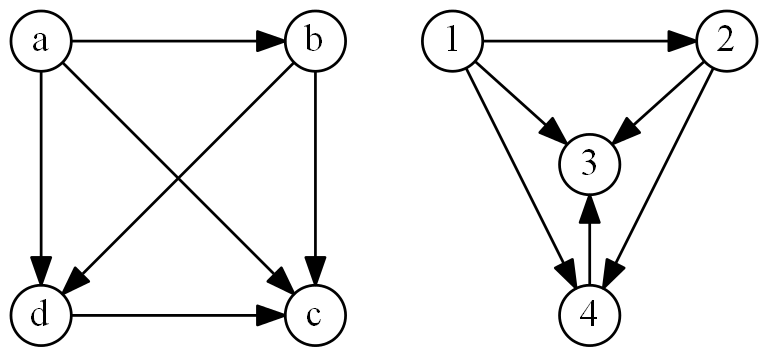
\includegraphics[width=10cm]{img/graph_izomorph.png}
	\end{center}
	\caption{Primer izomorfnih grafov z bijektivno funkcijo $f = \{(a, 1), (b, 2), (c, 3), (d, 4)\}$.}
	\label{pic_iso}
	\end{figure}


	Graf $G_p$ je izomorfen podgraf grafa $G_t$, če obstaja podgraf $G_t'$ grafa $G_t$, ki je izomorfen grafu $G_p$.
	Med grafoma $G_p$ in $G_t$ obstaja parcialen podgrafni izomorfizem, če je funkcija $f: V_p \to V_t$ injektivna in velja
	$(a,b) \in E_p \Rightarrow (f(a), f(b)) \in E_t$.
	Med grafoma $G_p$ in $G_t$ obstaja induciran podgrafni izomorfizem, če je funkcija $f: V_p \to V_t$ injektivna in velja
	$(a,b) \in E_p \Leftrightarrow (f(a), f(b)) \in E_t$. Na sliki~\ref{pic_sub_iso} vidimo, da je med $b)$ in $c)$ samo parcialni podgrafni
	izomorfizem, ker v vzorčnem grafu ni povezave $(B, C)$, medtem ko preslikavi teh vozlišč $(2, 3)$ tvorita povezavo v $c)$. Induciran 
	podgrafni izomorfizem lahko obstaja samo, če se ohranijo tudi ne-povezave.
	
	\section{Problem izomorfnega podgrafa}
	Obstajajo štiri različice problema izomorfnega podgrafa.
	\begin{itemize}
		\item{Odločitveni problem: ugotovi obstoj izomorfnega podgrafa.}
		\item{Preštevalni problem: ugotovi število izomorfnih podgrafov.}
		\item{Iskalni problem: poišči en izomorfen podgraf (preslikavo $f$).}
		\item{Naštevalni problem: poišči vse izomorfne podgrafe (preslikave $f$).}
	\end{itemize}
	Najtežje je iskanje vseh možnih preslikav -- to različico rešujejo opisani algoritmi. Dodatno lahko rešujemo
	problem še na usmerjenih ali neusmerjenih ter označenih ali neoznačenih grafih.


	\begin{figure}
	\begin{center}
	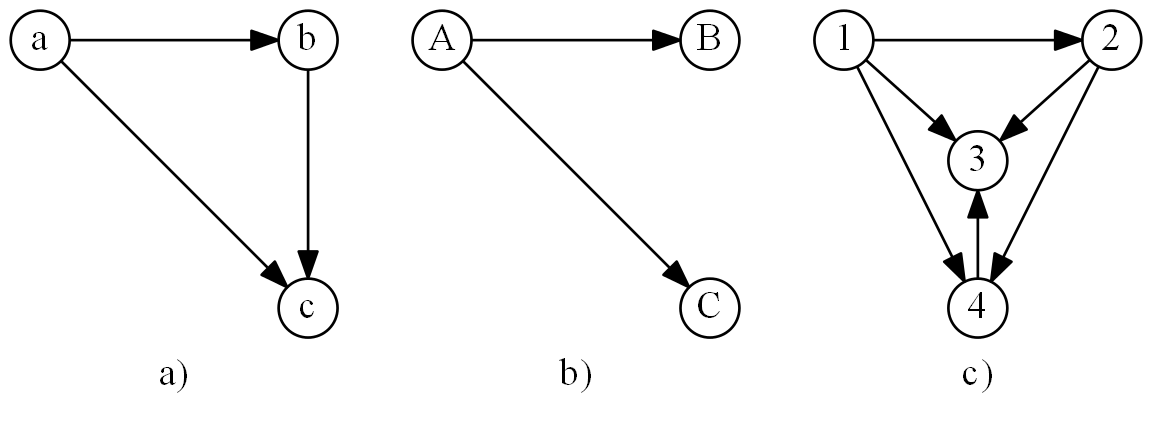
\includegraphics[width=15cm]{img/graph_sub_izomorph.png}
	\end{center}
	\caption{Med $a)$ in $c)$ obstaja induciran podgrafni izomorfizem z injektivno funkcijo $f = \{(a, 1), (b, 2), (c, 3)\}$. Med $b)$ in $c)$ obstaja
	samo parcialen podgrafni izomorfizem z injektivno funkcijo $f = \{(A, 1), (B, 2), (C, 3)\}$.}
	\label{pic_sub_iso}
	\end{figure}



	\section{Druge definicije}
	Na tem mestu so zbrane pomožne definicije, ki jih uporabljamo pri opisih algoritmov za iskanje izomorfnih podgrafov.

	V neusmerjenem grafu je število povezav, ki vsebujejo vozlišče $v$, stopnja (angl.~degree) vozlišča $v$. Označimo jo z $d(v)$. Množica vozlišč
	$N(v) = \{u \in V \big| \{v, u\} \in E\}$ je množica sosedov vozlišča $v$. 
	Množica sosednjih vozlišč podgrafa $S = (V_S, E_S)$ je definirana kot 
	$N(S) = \{ n \in V \setminus V_S \big| \exists m \in V_S : \{n,m\} \in E \}$. 

	V usmerjenem grafu je število povezav, ki imajo vozlišče $v$ za začetek
	povezave, 	izhodna stopnja (angl.~out-degree) vozlišča. Označimo jo z $d^+(v)$.
	Število povezav, ki imajo vozlišče $v$ za konec povezave, je vhodna stopnja (angl.~in-degree) vozlišča $v$. Označimo jo z $d^-(v)$.
	Množica naslednikov
	$N^+(v) = \{u \in V \big| (v,u) \in E\}$
	so končna vozlišča povezav, ki imajo za začetek povezave vozlišče $v$.
	Množica predhodnikov 
	$N^-(v) = \{u \in V \big| (u,v) \in E\}$
	so začetna vozlišča povezav, ki imajo za konec povezave vozlišče $v$. 
	Množica izhodnih sosedov (angl.~out-neighbors) podgrafa $S = (V_S, E_S)$ je definirana kot 
	$N^+(S) = \{ n \in V \setminus V_S \big| \exists m \in V_S : (m,n) \in E \}$.
	Množica vhodnih sosedov (angl.~in-neighbors) podgrafa $S = (V_S, E_S)$ je definirana kot 
	$N^-(S) = \{ n \in V \setminus V_S \big| \exists m \in V_S : (n,m) \in E \}$.

	Rez grafa $G$ je razdelitev vozlišč $V$ v dve disjunktni množici $(A, \bar A)$. Množico povezav, kjer je en konec povezave v $A$ in drugi v
	 $\bar A$, označimo z $e(A, \bar A) = \{(u,v) \in E \big| u \in A, v \not \in A\}$. Minimalna bisekcija  grafa G je rez, ki minimizira velikost reza 
	$| e(A, \bar A) |$ po vseh množicah $A$ velikosti $\lceil | V | / 2 \rceil$.



	\section{Zahtevnost problema}
	Odločitveni problem izomorfnega podgrafa spada v razred NP-polnih problemov~\cite{npcomplete}. Za dokaz NP-polnosti nanj prevedemo odločitveni
	problem iskanja polnega podgrafa oz. klike (angl.~clique problem). Pri slednjem, ki je znano NP-poln, imamo podan graf $G$ in
	število $k$, preverjamo pa obstoj polnega podgrafa s $k$ vozlišči (v polnem grafu obstaja povezava med vsakim parom vozlišč). Ta problem lahko rešimo 
	z iskanjem izomorfnega podgrafa tako, da najprej generiramo poln graf $H$ s $k$ vozlišči, nato pa preverimo, če v $G$ obstaja podgraf, ki je izomorfen
	$H$. Ker je problem iskanja polnega podgrafa NP-poln in smo ga v polinomskem času prevedli na problem iskanja izomorfnega podgrafa, je tudi 
	slednji problem NP-poln.






\chapter{Ullmannov algoritem}
	
	Prvi algoritem za iskanje podgrafnih izomorfizmov je J. R. Ullmann predstavil leta 1976. Kljub starosti se algoritem še vedno množično uporablja
	in je tudi najbolj znan. Celoten princip preiskovanja temelji na predstavitvi z matrikami. V osnovni verziji algoritem ne upošteva lokalne strukture
	vzorčnega grafa, s čimer npr. druga dva opisana algoritma hitreje izločata neobetavne poti preiskovanja.
	
	\section{Predstavitev problema podgrafnega izomorfizma z matrikami}
	V tem algoritmu predstavimo grafe in problem reševanja podgrafnih izomorfizmov z matrikami. Matriki $P = [p_{i,j}] : 1 \le i,j \le n_p $ in
	$T = [t_{i,j}] = 1 \le i,j \le n_t$ sta matriki sosednosti grafov $G_p$ in $G_t$, kjer vrednost 1 v vrstici $i$ in stolpcu $j$ pomeni, 
	da v grafu obstaja povezava
	iz $i$ v $j$:
		\begin{equation}
		 	p_{i,j} = \left\{
			\begin{array}{l l}
			    1 & (i,j) \in E_p\\
			    0 & \text{sicer.}
			\end{array} \right.
		\end{equation}
	Matrika $M = [m_{i,j}]: 1 \le i \le n_p \wedge 1 \le j \le n_t$ predstavlja preslikavo $f: V_p \to V_t$. Vrednost 1 v v vrstici $i$ in stolpcu $j$ 
	pomeni preslikavo vozlišča
	$i \in V_p$ v $j \in V_t$:
		\begin{equation}
			m_{i,j} = \left\{
			\begin{array}{l l}
			    1 & f(i) = j\\
			    0 & \text{sicer.}
			\end{array} \right.
		\end{equation}
	Matrika $M$ je injektivna, če je v vsaki vrstici natanko ena 1 in v vsakem stolpcu največ ena 1. Samo preslikavo lahko lahko zapišemo v matrični obliki:
		\begin{equation}
			%C = [c_{i,j}] = M(MT)^T
			C = [c_{i,j}] = (M(MT)^T)^T
		\end{equation}
		%\TODO{
		%$$%\begin{equation}
			%\text{mogoce tako, zaradi usmerjenih grafov? } C = [c_{i,j}] = (M(MT)^T)^T
		%$$%\end{equation}
		%}
	$M$ predstavlja podgrafni izomorfizem iz $G_p$ v $G_t$, če je dobljena matrika C enaka matriki sosednosti P:
		\begin{equation}
			\label{eq:ullmann1}
			c_{i,j} = p_{i,j}\;\; \forall i,j \in [1, n_p]
		\end{equation}	 
	Podana enačba velja za inducirani izomorfizem, pri enostavnem izomorfizmu je pogoj $p_{i,j} \Rightarrow c_{i, j}$.
	
	Ullmannov algoritem v osnovi generira različne matrike $M$ in jih preverja s pogojem~(\ref{eq:ullmann1}). Vseh možnih matrik $M$ je
	$\frac{n_t!}{(n_t-n_p)!}$ (ob upoštevanju pogoja za injektivnost: točno ena 1 v vrstici in največ ena 1 v stolpcu), kar je preveč za izčrpno preiskovanje.
	Algoritem zato začne z pred-procesirano matriko $M^0$~(razdelek~\ref{eq:ullmann2}), na vsakem koraku pa jo še dodatno omeji
	~(razdelek~\ref{eq:ullmann3}).
	
	
	\section{Algoritem}
	Matriko $M$ generiramo postopoma, po korakih. V danem koraku nam vrednost $m_{i,j}^k$ pove, ali se vozlišče $i \in V_p$ lahko preslika 
	v $j \in V_t$ (ima vrednost $1$) ali ne	(ima vrednost $0$). Izhajamo iz začetne matike $M^0$. V generiranju te matrike upoštevamo dejstvo, da
	se lahko vozlišče $i$ preslika v $j$ samo, če je stopnja vozlišča v vzorčnem grafu manjša ali enaka stopnji vozlišča v ciljnem grafu:
		\begin{equation}
		\label{eq:ullmann2}
		m_{i,j}^0 = \left\{ 
		  \begin{array}{l l}
		    1 & \text{$d(i) \leq d(j)$}\\
		    0 & \text{sicer.}
		  \end{array} \right.
		\end{equation}
	Pri usmerjenih grafih mora pogoj  veljati tako za vhodno kot za izhodno stopnjo.
	
	V vsakem naslednjem koraku izberemo še neobiskano vrstico. V vrstici izberemo stolpec, ki ima vrednost 1 in še ni bil izbran v nobeni prejšnji vrstici.
	Vse ostale vrednosti v vrstici postavimo na 0
	in gremo v naslednji korak. Če stolpca z vrednostjo 1 v trenutni vrstici ni, se vrnemo v prejšnji korak in izberemo drug stolpec. Ko obdelamo vse vrstice,
	se preveri pogoj~(\ref{eq:ullmann1}).
	
	Algoritem je Ullmann v izvirnem članku~\cite{ullmann} opisal s stavki GOTO, zaradi česar je težje razumljiv. Tukaj ga podajamo v bolj pregledni obliki,
	ki je popravljena in bolj podrobna različica algoritma iz~\cite{zampelli-th}. Potrebujemo naslednje podatkovne strukture:
	\begin{itemize}
		\item spremenljivko $d$, ki označuje trenutno globino v preiskovalnem drevesu
		\item spremenljivko $k$, ki označuje trenutno izbrani stolpec
		\item binaren vektor $F = <F_1, \ldots, F_i, \ldots,  F_{n_p} > $, v katerem z vrednostjo 1 na $i$-tem mestu označimo, 
			da je bil stolpec $i$ že izbran, z njim zagotovimo injektivnost preslikave
		\item vektor $H = < H_1, \ldots, H_d, \ldots, H_{n_p} > $, kjer $H_d = j$ pomeni, da je na globini $d$ izbran stolpec $j$ - od tu 
			obnovimo spremenljivko $k$ pri sestopanju
		\item matriko $M$, ki predstavlja trenutno matriko združljivih parov
		\item vektor matrik $M_v = < M_1, \ldots, M_d, \ldots, M_{n_p} > $, kjer je matrika $M_d$ zadnja generirana matrika $M$ na globini $d$ - od
			tu obnovimo matriko $M$ pri sestopanju
	\end{itemize}

	Prevdokoda algoritma je podana v \refalg{alg:ullmann1}. V vrsticah 1--2 inicializiramo vse spremenljivke -- začnemo z začetno matriko $M^0$, 
	na globini 1 in brez izbranega stolpca. V vrstici 3 shranimo matriko $M$ za prvi korak - matriko vedno shranjujemo pred vstopom v naslednji korak. 	
	Zanka v vrstici 4 še izteče, ko sestopimo iz obdelave prve vrstice, torej ko v prvi vrstici zmanjka neobiskanih stolpcev. V vrstici 5 poskrbimo, da 
	algoritem sestopi, če ne najdemo ustreznega stolpca. V vrstici 6 preverimo, če v trenutni vrstici obstaja še neobiskan stolpec. Ta stolpec mora biti še
	neizbran v trenutni vrstici ($j > k$), biti združljiv s trenutno vrstico ($m_{d,j} = 1$) in ne sme biti izbran v	katerem od prejšnjih korakov ($F_j=0$;
	pogoj za injektivno preslikavo). Sama izbira stolpca poteka v vrsticah 8--10, ko vrednost $k$ postavimo na izbrani stolpec, v vrstici 7 pa preprečimo 
	sestopanje, saj bomo v naslednji ponovitve zanke ali povečali globino ali pa ostali na isti globini.
	V vrstici 11 postavimo vse neizbrane stolpce v vrstici na $0$, torej izbrani stolpec označimo tudi v matriki $M$. Pogoj v vrstici 12 zaenkrat ignorirajmo.
	Če nismo prišli do dna preiskovalnega
	drevesa (vrstica 13), gremo v naslednji korak (vrstica 14): shranimo zadnji izbrani stolpec na trenutni globini ($H_d \gets k$), stolpec označimo kot
	že izbranega ($F_k \gets 1$), povečamo globino ($d \gets d + 1$), resetiramo izbiro stolpca za naslednji korak ($k \gets 0$) in shranimo matriko $M$
	za naslednji korak ($M_d \gets M$; od tukaj bomo obnavljali matriko $M$ ob vračanju v tisti korak).
	Če smo obdelali že vse vrstice v matriki $M$, potem v vrstici 16 preverimo, če matrika ustreza pogoju~(\ref{eq:ullmann1}), torej če matrika predstavlja
	podgrafni izomorfizem. Če pogoj drži, jo ustrezno shranimo ali izpišemo. V vrstici 18 obnovimo matriko $M$. Tako bomo
	v naslednji ponovitvi zanke preverili, če je v zadnji vrstici še kakšen primeren stolpec. Vrstici 19 in 20, tako kot vrstico 12, zaenkrat preskočimo.
	Vrstice 21--24 skrbijo za sestopanje, ki se izvede, če v trenutni 
	vrstici ni nobenega primernega stolpca več. V vrstici 22 sprostimo zadnji izbrani stolpec ($F_k \gets 0$) in znižamo globino. Nato v vrstici 24 obnovimo
	matriko $M$ in v $k$ obnovimo nazadnje izbrani stolpec na tej globini.
	
\begin{algorithm}
\caption{Ullmannov algoritem}
\label{alg:ullmann1}
\begin{algorithmic}[1]
	\Require Matriki sosednosti $P$ in $T$, začetna matrika $M^0$
	\Ensure Vse $n_p \times n_t$ matrike $M$, ki predstavljajo preslikave podgrafnih izomorfizmov				
	\State $M \gets M^0; d \gets 1; H_1 \gets 0; k \gets 0; backtract \gets true$								
	\For{$i $ in$ [1, n_p]$} $F_i \gets 0;$ \EndFor													
	\State $M_1 \gets M^0$																	
	\While{$d \not = 0$}																		
		\State $backtrack \gets true$													
		\If{$(\exists j : j > k \wedge m_{d,j} = 1 \wedge F_j = 0)$}			
			\State $backtrack \gets false$
			\Repeat 
				\State $k \gets k +1$ 															
			\Until{$m_{d,k} = 1 \vee F_k = 1$}													
			\State $\forall j \not = k : m_{d,j} \gets 0$										\label{alg:ullmann1.11}
			\If { [ \Call{refine}{$M, P, T$} ] }
				\If {$d < n_p$}																	
					\State $H_d \gets k; F_k \gets 1; d \gets d+1; k \gets 0; M_d \gets M$
				\Else																			
					\If {$<$ condition(\ref{eq:ullmann1}) $>$}											
						\State $<$ store $M$ $>$
					\EndIf													
					%\If{$\exists j : j > k \wedge m_{d,j} = 1 \wedge F_j = 0$}								
						\State $M \gets M_d$		
					%\EndIf
				\EndIf
			\Else
				\State $M \gets M_d$
			\EndIf
		\EndIf
		
		\If{$backtract$}																		
			\State $F_k \gets 0; d \gets d-1;$													
			\If{$d > 0 $}																	
				\State $M \gets M_d; k \gets H_d;$												
			\EndIf
		\EndIf
	\EndWhile
\end{algorithmic}
\end{algorithm}

	Velik del podanega algoritma se ukvarja s sestopanjem in obnavljanjem stanja pri sestopanju. Zato v \refalg{alg:ullmann3} podajamo še rekurzivno 
	različico algoritma. V tej različici za sestopanje in obnavljanje stanja skrbi sama rekurzija in je potek algoritma bolj očiten. V vrsticah 1 in 2 je
	inicializacija, le da sedaj potrebujemo manj spremenljivk. V vrstici 3 začnemo preiskovanje na globini 1. V vrstici 6 shranimo trenutno matriko $M$,
	ki jo bomo obnavljali ob sestopanju (ponovno zaenkrat ignoriramo del v oglatih oklepajih). V vrstici 7 je zanka, ki preveri vse stolpce. Ko pridemo do
	ustreznega (vrstica 8), vse ostale stolpce postavimo na 0 (vrstica 9), in označimo stolpec kot izbran (vrstica 10). Če smo v zadnji vrstici matrike $M$,
	potem preverimo pogoj~\ref{eq:ullmann1} in če smo našli izomorfizem, shranimo trenutno matriko $M$ (vrstice 11-13). Če to ni zadnja vrstica, gremo
	v naslednji korak (vrstica 15). Ob sestopanju obnovimo matriko $M$ in označimo trenutni stolpec kot neizbran (vrstica 16).

\begin{algorithm}
\caption{Ullmannov algoritem - rekurzivna različica}
\label{alg:ullmann3}
\begin{algorithmic}[1]
	\Require Matriki sosednosti $P$ in $T$, začetna matrika $M^0$
	\Ensure Vse $n_p \times n_t$ matrike $M$, ki predstavljajo preslikave podgrafnih izomorfizmov				
	\State $M \gets M^0$
	\For{$i $ in$ [1, n_p]$} $F_i \gets 0;$ \EndFor
	\State $step(1)$
%	\Statex
	\Subalg{\Call{step}{$d$}}
%	\Procedure{step}{d}
		\If { [\;!\,\Call{refine}{$M, P, T$} ] }
		%\If{$[! \; refine(M, P, T)\; ]$}
			\State \Return
		\EndIf
		\State $M_d \gets M$
		\ForAll{$k \in [1,n_t]$}
			\If{$m_{d,k} = 1 \wedge F_k = 0$}
				\State $\forall j \not = k : m_{d,j} \gets 0$
				\State $F_k \gets 1$
				\If{$d = n_p$}
					\If {$<$ condition(\ref{eq:ullmann1}) $>$}
						\State $<$ store $M$ $>$
					\EndIf
				\Else
					\State \Call{step}{$d+1$}
				\EndIf
				\State $F_k \gets 0; M \gets M_d$
			\EndIf
		\EndFor
%	\EndProcedure
\end{algorithmic}
\end{algorithm}


	\section{Omejevanje prostora preiskovanja}
	Ullmann je opazil, da lahko z dodatnim procesiranjem matrike $M$ na vsakem koraku dodatno omejimo prostor preiskovanja, torej da več 1 postavimo
	na 0. Če se bo vozlišče $i$ v preslikalo v vozlišče $j$, potem se mora tudi vsako sosednje vozlišče vozlišča $i$ preslikati v eno od 
	sosednjih vozlišč vozlišča $j$. Za vsak $m_{i,j} = 1$ preverimo pogoj:
	\begin{equation}
	\label{eq:ullmann3}
	\begin{array}{rcl}
	\forall x \in N_{p}(i) & \Rightarrow & \exists y \in N_t(j) \wedge m_{x,y} = 1
	\\
	\forall x \in [1, n_p] : p_{i,x} = 1 & \Rightarrow & \exists y \in [1, n_t] : t_{j,y} = 1 \wedge m_{x,y} = 1
	\end{array}
	\end{equation}
	Če pogoj ni izpolnjen, postavimo vrednost $m_{i,j}$ na 0. Vsaka sprememba v matriki lahko vpliva na pogoj pri ostalih vozliščih, zato postopek
	ponavljamo, dokler pri pregledu celotne matrike ne naredimo nobene spremembe. Ta pogoj je hkrati tudi zadosten za preverjanje podgrafnega 
	izomorfizma, zato lahko v algoritmih z njim nadomestimo pogoj~(\ref{eq:ullmann1}).
	
	Psevdokoda postopka je podana v~\refalg{alg:ullmann2}. Za vsak
	združljiv par (vrstica 4) preverimo pogoj~(\ref{eq:ullmann3}) v vrstici 5. Če pogoj ni izpolnjen, označimo par kot nezdružljiv (vrstica 6). Poleg tega
	označimo, da bo celoten postopek potrebno ponoviti ($fixpoint \gets false$). Ob spremembi v matriki $M$ preverimo še, če trenutna vrstica sedaj vsebuje
	same 1 (vrstica 7). V tem primeru namreč izomorfizem ni več mogoč, zato vrnemo $false$ (vrstica 8). Za opisani postopek je Ullmann predlagal tudi
	implementacijo z namenskim logičnim vezjem~\cite{ullmann}.

	Podani algoritem je v \refalg{alg:ullmann1} in \refalg{alg:ullmann3} že vključen, klic funkcije $refine$ je v oglatih oklepajih, ki smo jih predhodno
	ignorirali.

%\begin{spacing}{1} 
\begin{algorithm}
\caption{Omejevanje prostora}
\label{alg:ullmann2}
\begin{algorithmic}[1]
	\Require Matrika $M$ in sosednostni matriki $P$ in $T$
	\Ensure $true$ če je bila M omejena, $false$ če kakšna vrstica ne vsebuje nobene 1
	\Procedure{refine}{$M$, $P$, $T$}
		\Repeat
			\State $fixpoint \gets true$
			\For{$\forall (i,j): m_{i,j} = 1$}
				\If{condition (\ref{eq:ullmann3}) is not satisfied}
					\State $m_{i,j} \gets 0; fixpoint \gets false;$
					\If{$\forall k : m_{i,k} = 0$}
						\State \Return false
					\EndIf
				\EndIf
			\EndFor
		\Until{$fixpoint$}
		\State \Return $true$
	\EndProcedure
\end{algorithmic}
\end{algorithm}
%\end{spacing}

	\section {Časovna in prostorska zahtevnost}
	Prostorska zahtevnost celotnega algoritma je $O(n_p^2 n_t)$. Na vsaki globini shranimo matriko $M$, ki je velikosti $n_p n_t$, maksimalna globina pa 
	je $n_p$. Časovna kompleksnost funkcije $refine$ je $O(n_p n_t d_{max})$, kjer je $d_{max}$ največja možna stopnja vozlišča. Pogoj preverjamo za
	vsak	element matrike $M$, časovna zahtevnost pogoja pa je $d_{max}$, ker preverjamo samo sosede. Postopek preverjanja se sicer ponavlja do fiksne
	točke, ampak vsaka ponovitev dodatno poreže preiskovalno drevo, zato je ena ponovitev najslabši primer. Celoten algoritem ima časovno zahtevnost
	%$O(n_p! n_p n_t d_{max})$. 
	$O(n! n^2 d_{max})$. V posamezni ponovitvi zanke je funkcija $refine$ najzahtevnejša, število ponovitev pa je reda $n!$.


	\section{Izboljšave}
	\label{ull_imp}
	Ullmannov algoritem je v testih pokazal slabše rezultate od kasneje razvitih algoritmov \cite{vf2_2}. Leta 2012 pa sta Jurij Mihelič in Uroš Čibej predlagala
	več možnih izboljšav algoritma \cite{ull+}.
	
	V \refalg{alg:ullmann1} obiskujemo vozlišča iz vzorčnega grafa po vrsti, glede na sam zapis grafa z matriko. Drugačen vrsti red obiskovanja lahko
	pohitri algoritem, če čim hitreje ustavi preiskovanje poddreves, ki nimajo rešitve. Nekaj možnih hevristik:
	\begin{itemize}
	\item Najprej vozlišča z večjo stopnjo -- taka vozlišča imajo običajno manj kandidatov za preslikavo.
	\item Preiskovanje v širino, znotraj iste globine pa po stopnji
	\item Najboljši najprej -- začnemo z vozliščem z največjo stopnjo, v vsakem naslednjem koraku pa med sosedi že obiskanih vozlišč izberemo vozlišče z
	največjo stopnjo.
	\end{itemize}
	
	Omejevanje prostora iskanja s funkcijo $refine$ izkorišča dejstvo, da mora za vsakega soseda vozlišča $i$ obstajati združljiv sosed vozlišča $j$.
	Podobno pa velja, če še $i$ preslika v $j$, potem sosedje vozlišča $i$ ne morejo biti združljivi z vozlišči, ki niso sosedje vozlišča $j$:
	\begin{equation}
	\label{eq:ullmann_imp1}
	\forall x \in N_p(i) \;\; \forall y \not \in N_t(j) : m_{x,y} = 0
	\end{equation}
	Pri iskanju induciranega podgrafnega izomorfizma pa tudi v nasprotno smer:
	\begin{equation}
	\label{eq:ullmann_imp2}
	\forall y \in N_t(j) \;\; \forall x \not \in N_p(i) : m_{x,y} = 0
	\end{equation}
	Ta postopek lahko za razliko od $refine$ uporabimo samo za tiste $(i, j)$, za katere vemo, da bo $m_{i,j}$ obdržala vrednost 1. V \refalg{alg:ullmann1}
	bi ga uporabili v vrstici \ref{alg:ullmann1.11} nad $m_{d,k}$. Postopek zmanjša prostor preiskovanja za sosednja vozlišča, kar lahko dobro izkoristita 
	zadnji dve hevristiki iz prejšnjega odstavka. Pri njiju bodo namreč sosednja vozlišča hitro na vrsti za preiskovanje.
	
	Izboljšati je mogoče tudi prostorsko zahtevnost. Osnovni algoritem namreč na vsakem koraku shrani celotno matriko $M$. Namesto sklada matrik lahko
	uporabimo persistentno matriko. Ob spremembi vrednosti v matriki iz 1 v 0 na sklad shranimo koordinate spremembe. Ob sestopanju iz sklada
	preberemo koordinate sprememb in na ustreznih mestih vrednost povrnemo nazaj v 1. Ker je sprememb kvečjemu $n_p n_t$, se prostorska
	zahtevnost zmanjša na $O(n_p n_t)$.






\chapter{Algoritem VF2}
	
	Algoritem VF2~\cite{vf2, vf2_2} je novejši algoritem iz leta 2000. Izomorfizem išče iz delne rešitve, ki jo postopoma gradi z dodajanjem sosednjih vozlišč.
	Številka 2 v imenu pomeni posodobljeno verzijo, s katero so zmanjšali prostorsko zahtevnost~\cite{vf2_3}.

	Cilj algoritma VF2 je zgraditi preslikavo $M = \{(n,m) \in N_p \times N_t\}$. Medtem ko Ullmannov algoritem generira in preveri vse možne preslikave
	$M$, jih ta algoritem gradi postopoma. V vsakem stanju $s$ algoritma imamo parcialno preslikavo $M(s)$. Ta definira podgrafa $G_p(s) \subseteq G_p$ 
	in $G_t(s) \subseteq G_t$, ki sta si izomorfna in vsebujeta tista vozlišča, ki so tudi v $M(s)$. Uporabljali bomo oznaki $M_p(s)$ in $M_t(s)$,
	ki predstavljata množico vozlišč v omenjenih podgrafih.	Prehod iz stanja $s$ v naslednje stanje $s'$ predstavlja razširitev trenutne $M(s)$ z dodatnim
	parom vozlišč. Nov par $(n, m)$ izberemo med sosedi $G_p$ in $G_t$ tako, da tudi razširjena $M(s')$ definira izomorfna podgrafa.
	
	Psevdokoda okvirnega poteka algoritma je podana v~\refalg{alg:vf2}. Algoritem je rekurziven in preiskuje z globino. Ob prvem klicu je $M(s_0)$ prazna.
	V vrstici 2 preverimo,
	če $M(s)$ že pokriva celoten vzorčni graf. Ker $M(s)$ po konstrukciji predstavlja izomorfizem, smo v tem primeru že našli pografni izomorfizem med
	$G_p$ in $G_t$, zato $M$ izpišemo. V vrstici 5 izračunamo vse možne kandidate za razširitev $M(s)$, kjer kandidate izbiramo med sosedi trenutnih
	podgrafov. Podrobnejši opis je v razdelku~\ref{vf2:candidate}. V vrsticah 6--9 za vsak par preverimo, če je združljiv. Pri tem uporabljamo pravila, ki so
	opisana v razdelku~\ref{vf2:feasible}. Če je par ustrezen, z njim razširimo $M(s)$ (s čimer dobimo $s'$) in rekurzivno kličemo algoritem nad novim
	stanjem.

\begin{algorithm}
\caption{Algoritem VF2}
\label{alg:vf2}
\begin{algorithmic}[1]
	\Require Vmesno stanje $s$, začetno stanje $s_0$ ima $M(s_0) = \emptyset $
	\Ensure Vse preslikave podgrafnih izomorfizmov
	\Procedure{vf2}{$s$}
		\If{ $M(s)$ covers all $G_p$}
			\State output $M(s)$
		\Else
			\State Generate candidates $P(s)$
			\ForAll{$p \in P(s)$}
				\If{$feasible(p)$}
					\State Compute $s'$ by adding $p$ to $M(s)$
					\State \Call{vf2}{$s'$}
				\EndIf
			\EndFor
		\EndIf
		\State restore data structures
	\EndProcedure
\end{algorithmic}
\end{algorithm}



	\section{Izbira kandidatov}
	\label{vf2:candidate}
	
	Množico kandidatov $P(s)$ izbiramo med neposrednimi sosedi podgrafov $G_p(s)$ in $G_t(s)$. Naj bosta $T_p^+(s)$ in $T_t^+(s)$ množici vozlišč iz
	$G_p$ in $G_t$ , ki še niso v preslikavi $M(s)$ in so izhodni sosedi katerega izmed vozlišč v $M(s)$. Podobno naj bosta $T_p^-(s)$ in $T_t^-(s)$ množici
	vozlišč, ki še niso v preslikavi $M(s)$ ter imajo izhodne sosede v $M(s)$. V množico $P(s)$ sestavljajo pari $(n,m)$, kjer velja $n \in T_p^+(s) \wedge
	m \in T_t^+(s)$. Če takega para ni, se upoštevata množici $T_p^-$ in $T_t^-$. Če tudi takega para ni, upoštevamo vsa vozlišča, ki še niso v preslikavi
	$M(s)$. Slednji primer se zgodi, če je graf sestavljen iz več nepovezanih delov in čisto na začetku, ko je $M(s)$ prazna. $P(s)$ torej postane ena od
	naslednjih množic:
	\begin{enumerate}
	\item $T^+(s) = \{min\; N^+(M_p(s))\} \times N^+(M_t(s))$
	\item $T^-(s) = \{min\; N^-(M_p(s))\} \times N^-(M_t(s))$\;\;\; če je $T^+(s)$ prazna
	\item $P^d(s) = \{min\; (V_p \setminus (M_p(s) \cup T_p(s))) \}  \times (V_t \setminus (M_t(s) \cup T_t(s)) )$\;\;\; če je $T^-(s)$ prazna
	\end{enumerate}
	
	Primer opisanih množic je na sliki~\ref{pic_t_in_out}. Če bo algoritem iz trenutnega stanja prišel do konca (torej bo našel podgrafni izomorfizem), mora
	obstajati preslikava za vsak element iz vzorčnega grafa. Zato je dovolj, da v parih, ki jih vstavimo v množico $P(s)$ nastopa samo eno vozlišče iz
	vzorčnega grafa. Če algoritem ne bo našel podgrafnega izomorfizma z uporabo tega vozlišča, ga ne bo tudi z nobenim drugim. Zato iz vzorčnega grafa 
	vzamemo vedno samo najmanjši element, kar predstavlja oznaka $min$ v enačbah. Na tak način se tudi izognemo generiranju enakih stanj. Podobno 
	razmišljanje nas privede do zaključka, da lahko prekinemo trenutno pot preiskovanja, če je $T_t^+$ prazna, $T_p^+$ pa ne (in isto za $T_t^-$,
	$T_p^-$). 	Omenimo še, da v sami implementaciji algoritma ni potrebe po eksplicitnem generiranju $P(s)$.
	
	\begin{figure}
	\begin{center}
	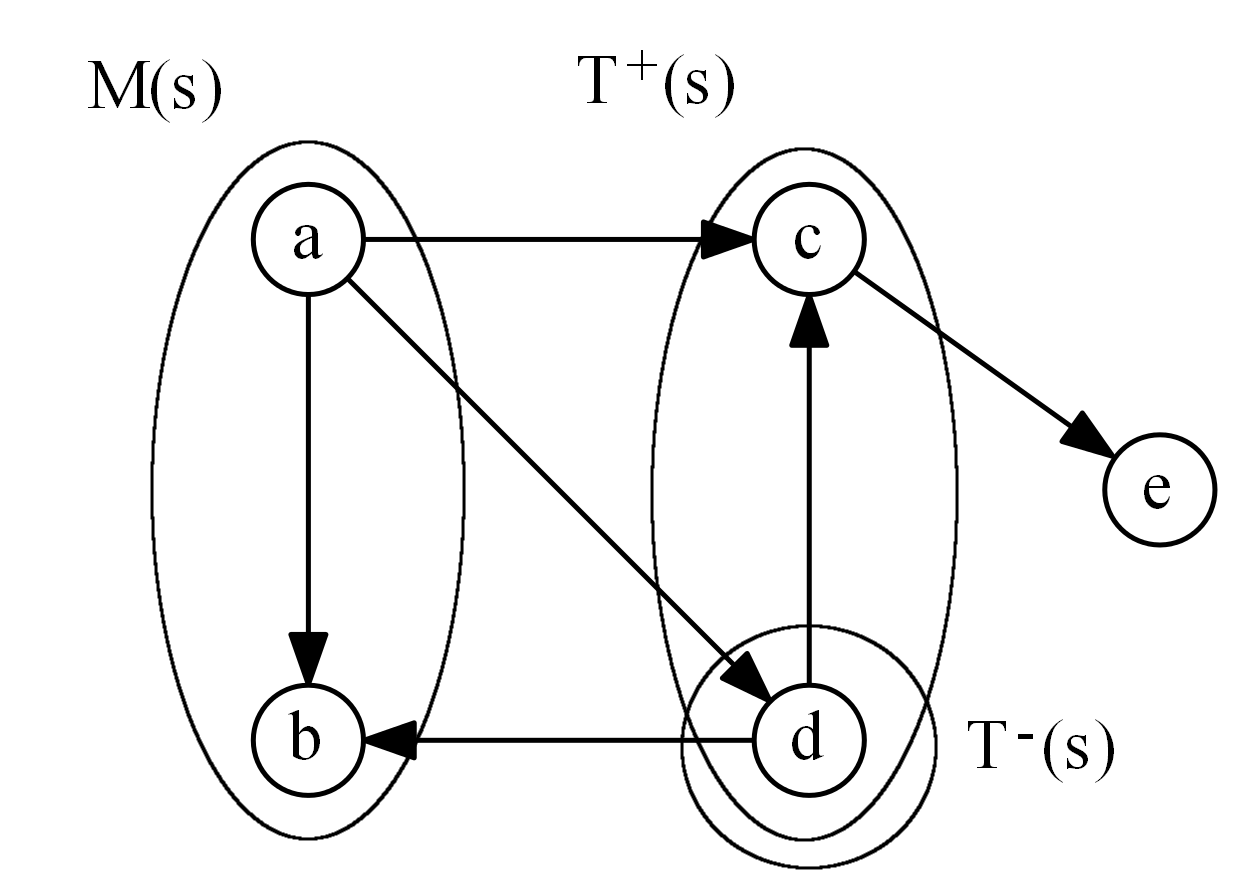
\includegraphics[width=8cm]{img/graph_t_in_out.png}
	\end{center}
	\caption{}
	\label{pic_t_in_out}
	\end{figure}



	\section{Izračun združljivosti kandidatov}
	\label{vf2:feasible}

	Pri preverjanju posameznega para $(n,m)$ iz $P(s)$ upoštevamo pet pravil. Z enačbama ~\ref{eq:vf2r1} in \ref{eq:vf2r2} preverimo, da bo razširjena
	parcialna preslikava še vedno predstavljala izomorfizem obdelanih podgrafov. Vsak sosed vozlišča iz vzorčnega grafa v parcialni preslikavi se mora
	preslikati v soseda vozlišča iz ciljnega grafa. Pogoj ločimo za vhodne in izhodne sosede. V oglatih oklepajih je zapisan
	še obratni pogoj, ki mora veljati pri iskanju induciranega podgrafa.
	\begin{equation}
	\label{eq:vf2r1}
	\begin{array}{rcl}
	(\forall n' \in N_p^-(n) \cap M_p(s) \; \exists m' \in N_t^-(m)    \!\!\!&:&\!\!	 (n', m') \in M(s)) \\
	\;[\; \wedge \; (\forall m' \in N_t^-(m) \cap M_t(s)\; \exists n' \in N_p^-(n) \!\!\!&:&\!\! (n', m') \in M(s)) \;]
	\end{array}
	\end{equation}
	\begin{equation}
	\label{eq:vf2r2}
	\begin{array}{rcl}
	(\forall n' \in N_p^+(n)  \cap M_p(s)  \; \exists m' \in N_t^+(m)    \!\!\!&:&\!\!	 (n', m') \in M(s)) \\
	\;[\; \wedge \; (\forall m' \in N_t^+(m) \cap  M_t(s)\; \exists n' \in N_p^+(n)     \!\!\!&:&\!\!	 (n', m') \in M(s)) \;]
	\end{array}
	\end{equation}
	
	Ta pogoj je zadosten za pravilno preiskovanje, z dodatnimi pogoji pa dodatno skrčimo prostor preiskovanja. Preverjamo število sosedov v posameznih 
	množicah.  Prejšnji enačbi že preverjata sosede iz množice $M(s)$. Z enačbama~\ref{eq:vf2r3} in \ref{eq:vf2r4} preverjamo število sosedov v
	množici $T(s)$. Posebej preverimo za $T^-(s)$ in $T^+(s)$ ter za vhodne in izhodne sosede. Število sosedov mora v vzorčen grafu biti manjše ali
	enako število sosedov v ciljnem grafu.
	\begin{equation}
	\label{eq:vf2r3}
	\begin{array}{rcl}
	|N_p^-(n) \cap T_p^-(s)|   \! & \! \leq \! & \! |N_t^-(m) \cap T_t^-(s)| \; \wedge \\
	|N_p^+(n) \cap T_p^-(s)|  \! & \! \leq \! & \! |N_t^+(m) \cap T_t^-(s)|
	\end{array}
	\end{equation}
	\begin{equation}
	\label{eq:vf2r4}
	\begin{array}{rcl}
	|N_p^-(n) \cap T_p^+(s)|   \! & \! \leq \! & \! |N_t^-(m) \cap T_t^+(s)| \; \wedge \\
	|N_p^+(n) \cap T_p^+(s)|  \! & \! \leq \! & \!|N_t^+(m) \cap T_t^+(s)|
	\end{array}
	\end{equation}
	
	Enačba~\ref{eq:vf2r5} preveri še število sosedov, ki niso v množici $M(s)$ ali $T(s)$, torej sosede iz množice $P^d(s)$.
	\begin{equation}
	\label{eq:vf2r5}
	\begin{array}{rcl}
	|N_p^-(n) \setminus (M_p(s) \cup T_p(s))| \! & \! \leq \! & \! |N_t^-(n) \setminus (M_t(s) \cup T_t(s))| \; \wedge \\
	|N_p^+(n) \setminus (M_p(s) \cup T_p(s))| \! & \! \leq \! & \! |N_t^+(n) \setminus (M_t(s) \cup T_t(s))|
	\end{array}
	\end{equation}
	
	Pri grafih z oznakami enačbi~\ref{eq:vf2r1} dodamo še pogoj kompatibilnosti oznak povezav, oznake vozlišč pa lahko preverjamo že pri izgradnji
	množice $P(s)$.



	\section{Časovna in prostorska zahtevnost}
	\label{vf2:impl}
	Za hitro izvajanje algoritma in čim manjšo porabo prostora je pomembna ustrezna izbira podatkovnih struktur. Implementacija avtorjev algoritma	
	poleg podatkovnih struktur za hrambo grafov
	uporablja šest vektorjev. Parcialno preslikavo $M(s)$ predstavljata vektorja \code{core\_p} in \code{core\_t}. Če $(n,m) \in M(s)$, potem
	ima \code{core\_p[n]} vrednost $m$ in \code{core\_t[m]} vrednost $n$. V nasprotnem primeru imata oba vrednost $null$. Množice $T_p^-$, 
	$T_p^+$, $T_t^-$, $T_t^+$ predstavimo z vektorji \code{in\_p}, \code{out\_p}, \code{in\_t}, \code{out\_t}. Vrednost \code{in\_p[n]} je 
	pozitivna, če velja $n \in T_p^- \; \vee \; n \in M_p(s)$, drugače je $null$. Podobno so definirane tudi ostale množice. Za ekskluzivno pripadnost
	vozlišča $n$ množici $T_p^-$ mora veljati \code{in\_p[n] > 0} in \code{core\_p[n] == null}.
	
	Omenjene vektorje si vsa stanja preiskovanja delijo. Velja namreč, da ob prehodu v novo stanje zapise v vektorjih samo dodajamo, oz. jim spreminjamo
	vrednosti iz $null$ v neko pozitivno vrednost. Ob sestopanju jih lahko zato obnovimo. Vektorjema \code{core} spremenimo vsakemu samo eno vrednost 
	in si to vrednost zapomnimo. Pri ostalih vektorjih je ob spremembi pomembno samo, da imajo vrednost večjo od 0. Lahko jim damo vrednost, ki ustreza
	trenutni globini preiskovanja. Ob sestopanju izbrišemo vrednosti s trenutno globino. Pri tem tudi ni potreben obhod celotnega vektorja,
	ampak je zadosti, da preverimo samo sosede izbranega para. Samo za ta vozlišča je namreč bila sprememba možna.
	Tako ni potrebe po hranjenju kopije vektorja pri vsakem stanju. Ker velja $n_t \geq n_p$, je torej prostorska zahtevnost celotnega algoritma $O(n_t)$.
	
	V najslabšem primeru bo algoritem moral zgenerirati vse možna stanja, ki jih je reda $n!$. Vsako stanje mora izračunati tri stvari:
	\begin{itemize}
	\item Preveri, če držijo pravila iz razdelka~\ref{vf2:feasible}. To je možno narediti z enim prehodom po vseh sosedih izbranega para, vse
	potrebne operacije pa se zaradi izbranih podatkovnih struktur izvedejo v konstantnem času. Časovna zahtevnost tega dela je torej $O(d_p(n) + d_t(m))$.
	\item Izračuna nove množice $T_p^-$, $T_p^+$, $T_t^-$, $T_t^+$. Tudi to lahko opravimo z enim prehodom po vseh sosedih, nastavljamo vrednost
	na tistih indeksih, ki vrednosti še nimajo. Časovna zahtevnost je isto $O(d_p(n) + d_t(m))$.
	\item Generiramo množico parov, ki so kandidati za vključitev v $M(s)$. Iz vzorčnega grafa vzamemo prvi element, ki v ustreznem vektorju (\code{in\_p},
	\code{out\_p}) še nima vrednosti. V množico dodamo še vse elemente iz komplementarne množice, te dobimo z enim prehodom ustreznega vektorja.
	Časovna zahtevnost je torej $O(n_t)$
	\end{itemize}
	Skupna časovna zahtevnost je zato $O(n!n)$






\chapter{Subsea}
	Algoritem Subsea~\cite{subsea} je najnovejši izmed predstavljenih algoritmov. Deluje po principu deli in vladaj:
	\begin{enumerate}
		\item Zgeneriramo vse zgodovine pregledov za vzorčni graf (razdelek~\ref{sub:th})
		\item Ciljni graf razbijemo z bisekcijo (aproksimacijski algoritem - razdelek~\ref{sub:bisect}).
		\item Na vsaki povezavi med obema deloma bisekcije preverimo obstoj podgrafnega izomorfizma z uporabo zgodovin pregledov 
			(razdelek~\ref{sub:search}).
		\item Na vsakem delu bisekcije ponovimo postopek od koraka 2 naprej; končamo, ko je ima posamezen del bisekcije manj vozlišč kot vzorčni graf.
	\end{enumerate}
	Pri samem iskanju uporabi hevristiko, ki poskuša čim hitreje najti negativne primere in končati iskanje v taki veji.
	
	Zaradi faze predprocesiranja se najbolje obnese pri iskanju vseh instanc podgrafov. Za razliko od prvih dveh algoritmov ima Subsea nekaj omejitev. 
	Dobro deluje predvsem, če je vzorčni graf mnogo manjši od ciljnega, poleg tega pa mora biti vzorčni graf povezan. Ker oboje drži za večino praktičnih
	problemov, omejitve niso posebno omejujoče. 

	\section{Bisekcija grafa}
	\label{sub:bisect}
	Algoritem Subsea med delovanjem razdeli graf na dve enako veliki množici (particiji) - naredi bisekcijo. Algoritem deluje hitreje, če je bisekcija 
	minimalna, torej če je število povezav med obema deloma grafov minimalno. Soroden problem je problem minimalnega reza, le da pri njem ni 
	pomembno število elementov v particijah. Problem minimalne bisekcije je NP-poln, vendar pravilnost algoritma Subsea ni odvisna od natančnosti
	minimalne bisekcije, zato se uporabljajo hitre aproksimacijske metode.

	Prva taka metoda je  algoritem ``črnih lukenj" (Black holes bisection). Začne s praznima particijama $B_1$ in $B_2$. Potem v vsako particijo izmenično
	dodaja po eno vozlišče.
	Vozlišče izbira med sosednjimi vozlišči trenutne particije. Torej v $B_1$ doda naključno vozlišče iz $V \setminus (B_1 \cup B_2)$, ki ima soseda v $B_1$.
	Podobno tudi za drugo particijo. Če takega vozlišča ni, doda naključno še ne izbrano vozlišče. Algoritem temelji na dejstvu, da če sta particiji (``črni 
	luknji") trenutno locirani na 	nasprotnih straneh minimalne bisekcije, bo več sosedov iz iste strani minimalne bisekcije in posledično večja verjetnost, da
	dodamo ustrezno vozlišče. Psevdokoda je podana v~\refalg{alg:sub_bh}.

\begin{algorithm}
\caption{Bisekcija grafa - ``črne luknje"}
\label{alg:sub_bh}
\begin{algorithmic}[1]
	\Require Graf $G = (V, E)$
	\Ensure Rez $(B, \bar B)$, ki je aproksimacija minimalne bisekcije
	\State $B_1 \gets B_2 \gets \emptyset$
	\State $B_0 \gets V \setminus (B_1 \cup B_2)$
	\Repeat
		\State \Call{Add2Hole}{$1$}
		\State \Call{Add2Hole}{$2$}
	\Until {$B_0 = \emptyset $}
	
	\Subalg{\Call{Add2Hole}{$i$}}

	\If {$B_0 = \emptyset$} \Return \EndIf
	\State $E_0 \gets \{ (u,v): u \in B_i, v \in B_0 \}$
	\If {$E_0 \not = \emptyset $}
		\State \textbf{choose randomly} $e = (u,v) \in E_0: v \in B_0$
	\Else
		\State \textbf{choose randomly} $v \in B_0$
	\EndIf
	\State $B_i \gets B_i \cup \{ v \}$
	\State $B_0 \gets B_0 \setminus \{ v \}$
\end{algorithmic}
\end{algorithm}

	Druga metoda je požrešni algoritem. Ta začne z že obstoječo bisekcijo, ki pa je lahko kar rezultat prve metode, ter jo lokalno optimizira. Za vsako vozlišče
	izračuna notranjo ceno $I(x)$, ki je število sosedov vozlišča $x$ znotraj iste particije, in zunanjo ceno $E(x)$, ki je število sosedov v drugi particiji. Potem
	za vsak par $x \in B$, $y \in \bar B$ izračuna spremembo cene reza ob morebitni zamenjavi para: $gain = E(x) - I(x) + E(y)  - E(y) - 2w(x,y)$, kjer
	$w(x,y) = 1$, če sta vozlišči povezani, in $w(x,y) = 0$ če vozlišči nista povezani ($w$ je korekcija morebitne medsebojne povezave - ta je zunanja in za
	razliko od ostalih tudi po zamenjavi ostane zunanja). Algoritem nato menja pare vozlišč z največjo pridobitvijo, pri vsaki zamenjavi pa popravi $I(v')$ 
	in $E(v')$ za vsakega soseda zamenjanega para. Ustavi se, ko ni več para z $gain > 0$.
	
	
	
	\section{Zgodovina pregleda grafa}
	\label{sub:th}
	%\TODO{sliki?}
	Algoritem Subsea med iskanjem podgrafnega izomorfizma ne uporablja vzorčnega grafa, ampak zgodovino pregleda. Ta enolično določa vrstni red
	obiskovanja vozlišč. Motivacija za tak pristop je, da v fazi predprocesiranja določimo vrstni red preiskovanja, ki bi čim hitreje ugotovil, da izomorfizem
	ni mogoč.
	
	Zaporedno številko obiskovanja označuje preslikava $d : V \to \mathbb{N}$. Za vsako vozlišče definiramo $l_i = l(v): d(v) = i$, ki je oznaka vozlišča,
	ki smo ga obiskali kot $i$-tega zaporednega. Definiramo še $N_i = \{ d(u) < i: u \in N_G(v) \, \wedge \, d(v) = i\}$, ki za $i$-to vozlišče predstavlja
	njegove sosede, ki smo jih že obiskali. Zgodovina pregleda grafa je zaporedje $\langle (l_1, N_1), (l_2, N_2), \ldots (l_{|V|}, N_{|V|})\rangle$. To
	zaporedje bomo kasneje uporabili za preverjanje izomorfizma v ciljnem grafu. Vozlišča bomo preiskovali v vrstnem redu, ki ga določa zgodovina pregleda
	v vzorčnem grafu. Za vsako obiskano vozlišče iz ciljnega grafa bomo preverili, če ustreza oznaki vozlišča iz zgodovine pregleda (ima enak $l_i$) in če
	struktura trenutnega podgrafa ustreza strukturi vzorčnega grafa ($N_i$ vzorčnega grafa mora biti podmnožica $N_i$ ciljnega grafa, oziroma morata biti
	množici enaki v primeru iskanja induciranega podgrafa). Če bi imeli usmerjene grafe, bi morali hraniti ločeni množici $N_i$ za vhodne in izhodne
	povezave.
	
	Psevdokoda algoritma, ki izračuna zgodovino pregleda z začetkom v dveh podanih vozliščih, je v~\refalg{alg:sub_th}. Deluje po principu preiskovanja
	v globino, pri čemer naslednje vozlišče izbere na podlagi hevristike. V vrsticah \ref{line:th1}--\ref{line:th4} inicializiramo potrebne podatkovne strukture
	in obiščemo prvo vozlišče. V vrstici \ref{line:th6} obiskanemu vozlišču določimo zaporedno številko. V vrstici \ref{line:th7} gradimo samo zgodovino
	pregleda grafa. V vrstici \ref{line:th7} zagotovimo, da kot drugega obiščemo vozlišče $v_2$. Začetek na vozliščih $v_1, v_2$ je potreben, ker moramo 
	zgenerirati zgodovino pregleda za vsako povezavo v vzorčnem grafu. V vrsticah \ref{line:th9}--\ref{line:th13} obiščemo vsa naslednja vozlišča. Kandidati
	so sosedi trenutnega vozlišča (vrstica \ref{line:th9}). Vrstni red določa hevristika (vrstica \ref{line:th11}). Najbolšega kandidata rekurzivno obiščemo
	(preiskovanje v globino, vrstica \ref{line:th12}) in odstranimo s seznama kandidatov (\ref{line:th13}).
	
	Hevristika daje prednost vozliščem, ki so tesno povezani z že pregledanimi vozlišči. Funkcija za izračun hevristike vrača par koordinat. Prva predstavlja
	število korakov ki jih potrebujemo iz kandidata $w$ do poljubnega že pregledanega vozlišča, pri čemer jasno ne smemo uporabiti povezave $(v, w)$.
	Druga koordinata predstavlja število že obiskanih vozlišč, ki jih s toliko koraki lahko dosežemo (to številko pomnožimo z $-1$). Med kandidati izberemo
	tistega z minimalnim parom koordinat, torej tistega, ki potrebuje najmanj korakov (je najbližje že pregledanim vozliščem), med izenačenimi pa tistega,
	preko katerega pridemo do največjega števila že obiskanih vozlišč.
	Koordinati izračunamo s preiskovanjem v širino. Začnemo z množico, v kateri je samo kandidat $w$, dolžina poti pa je $1$ (vrstici \ref{line:th14} in
	\ref{line:th15}). Nato v zanki opravljamo preiskovanje. V vrstici \ref{line:th17} izračunamo vse sosede trenutne množice $S$ (in ignoriramo omenjeno
	povezavo $(w,v)$). V vrstici \ref{line:th18} preštejemo, koliko že pregledanih vozlišč smo dosegli. Če smo dosegli vsaj enega, vrnemo rezultat v
	v vrstici \ref{line:th19}, drugače povečamo korak (vrstici \ref{line:th20} in \ref{line:th21}). Če ni več novih sosedov (vrstica \ref{line:th22}), pomeni,
	da iz $w$ ni mogoče doseči že pregledanih vozlišč, razen preko $v$. Take kandidate bomo pregledali nazadnje, zato prvo koordinato nastavimo na 
	$\infty$, drugo pa na velikost množice vozlišč, dosegljivih iz $w$.
	
\begin{algorithm}
\caption{Zgodovina pregleda grafa (angl.~Traverse history)}
\label{alg:sub_th}
\begin{algorithmic}[1]
	\Require Graf $G = (V, E)$, začetni vozlišči $v_1, v_2 \in V$, da velja $(v_1, v_2) \in E$
	\Ensure Zgodovina prehoda $H$ z začetkom v $v_1, v_2$

	\ForAll {$v \in V$}			\label{line:th1}
		\State $d(v) \gets 0$
	\EndFor
	\State $vtime \gets 1$
	\State \Call{Visit}{$v_1$}		\label{line:th4}
	\State \Return $H$


	\Subalg{\Call{Visit}{$v$}}
	\State $d(v) \gets vtime$ 		\label{line:th6}
	\State $H[vtime+\!+] \gets (l(v), \{0 < d(u_1) \leq \ldots \leq d(u_m) : u_1, \ldots, u_m \in N_G(v)\})$ 	\label{line:th7}
	\If {$v = v_1$}
		\Call{Visit}{$v_2$}						\label{line:th8}
	\EndIf
	\State $N_0 \gets \{ u \in N_G(v): d(u) = 0 \}$		\label{line:th9}
	\While {$N_0 \not = \emptyset$}					\label{line:th10}
		\State \textbf{choose} $w \in N_0$ with miminal \Call{EstimateNext}{$w, v$}		\label{line:th11}
		\If {$d(w) = 0$} 
			\Call{Visit}{$w$}					\label{line:th12}
		\EndIf
		\State $N_0 \gets N_0 \setminus \{w\}$		\label{line:th13}
	\EndWhile


	\Subalg{\Call{EstimateNext}{$w, v$}}
	\State $S \gets \{w\}$						\label{line:th14}
	\State $len \gets 1$							\label{line:th15}
	\Repeat
		\State $N_S \gets \cup_{z \in S}N_{G\, \setminus\,  (v,w)}(z)$	\label{line:th17}
		\State $p \gets | \{ y \in N_S: d(y) > 0 \} |$					\label{line:th18}
		\If {$p > 0$}										\label{line:th19}
			\Return $\langle len, -p \rangle$
		\EndIf
		\State $len+\!+$						\label{line:th20}
		\State $S \gets S \cup N_S$			\label{line:th21}
	\Until {$N_S \not = \emptyset$}				\label{line:th22}
	\State \Return $ \langle \infty, |S| \rangle $	\label{line:th23}
\end{algorithmic}
\end{algorithm}

	\clearpage


	\section{Iskanje izomorfnega podgrafa}
	\label{sub:search}
	Ko imamo zgodovino pregleda za ciljni glaf, jo uporabimo pri iskanju podgrafnega izomorfizma. Psevdokoda algoritma je podana v~\refalg{alg:sub_st}.
	Iskanje sprožimo nad konkretno povezavo v ciljnem grafu (glej razdelek~\ref{sub:subsea}). Deli v oglatih oklepajih veljajo za primer iskanja
	induciranega podgrafa. V vrsticah \ref{line:st1}--\ref{line:st4} inicializiramo preslikavo $g$ (v ciljnem grafu uporabljamo oznako $g$ namesto $d$,
	da se ju ne meša) in definiramo vrednosti v preslikavi za podani vozlišči. Tako omejimo preiskovanje v ciljnem grafu na samo tiste podgrafe, ki 
	vsebujejo podano povezavo. V vrstici \ref{line:st5} je prvi klic rekurzivne funkcije, ki bo od sedaj naprej sledila vrstnemu redu preiskovanja iz podane
	$H$.
	
	V funkcije $searchVisit$ naprej dobimo vrednost zadnje zaporedne številke iz $g$ in ustrezno vozlišče (zadnje dodano vozlišče, vrstici \ref{line:st6}
	in  \ref{line:st7}). Za to vozlišče v vrstici \ref{line:st8} preverimo, če ustreza vozlišču iz vzorčnega grafa z isto zaporedno številko, torej če je
	dodajanje tega vozlišča ohranilo izomorfizem trenutno pregledanega dela grafa. Veljati mora, da so vsa vozlišča v trenutni $N_i$ iz zgodovine
	pregleda $H$ vsebovana med pregledanimi sosedi dodanega vozlišča (primerjamo njihove preslikave iz $d$ oz.~$g$). Če to ne velja, ne podgrafnega
	izomorfizma ni, zato sestopimo. Za primer iskanja induciranega podgrafa morata biti omenjeni množici enaki (vrstica  \ref{line:st10}). Pri usmerjenih
	grafih pa bi ločeno preverjali množici vhodnih in izhodnih sosedov. V vrstici \ref{line:st12} v trenutni preiskani podgraf dodamo še povezave, ki
	pripadajo prej dodanemu vozlišču. Povezave potrebujemo, da lahko vrnemo celoten izomorfen podgraf, ko smo ga našli (vrstica  \ref{line:st13}).
	
	V drugem delu funkcije $searchVisit$ najdemo in pregledamo vse kandidate za naslednje dodano vozlišče. Iz $H[vtime + 1].N$ vemo, s katerimi že 
	pregledanimi vozlišči mora biti naslednje vozlišče povezano. Obratno torej velja, da so kandidati tista vozlišča, ki so sosednja vsem vozliščem iz 
	$H[vtime + 1].N$ (vrstica \ref{line:st14}). V vrsticah \ref{line:st17}--\ref{line:st20} te kandidate preverimo: če kandidat še ni bil obiskan, mu
	v preslikavi $g$ določimo naslednjo zaporedno številko in obiščemo novo stanje. Ob vrnitvi razveljavimo spremembo v $g$.
	
	V vrstici \ref{line:st17} je še dodaten pogoj, ki mora veljati v primerju iskanja induciranih podgrafov. Kot bomo videli v naslednjem razdelku, med
	procesom iskanja vseh podgrafnih izomorfizmov brišemo že obdelane povezave, s čimer preprečimo, da bi isti podgraf našli ponovno kasneje v
	procesu iskanja. Pri induciranih podgrafih pa povezave ne smemo brisati, ampak jo	označimo kot ``črno" (primer, zakaj je to potrebno, je na 
	sliki~\ref{pic_subsea_black}). Zato moramo pri kandidatu preveriti, da nima nobene ``črne" povezave na že pregledano vozlišče.
	
	\begin{figure}
	\begin{center}
	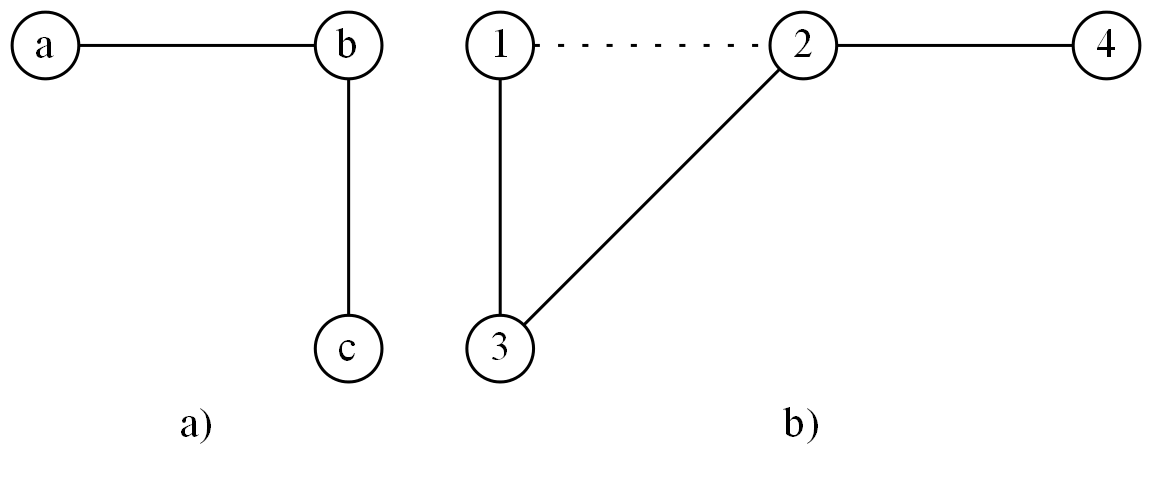
\includegraphics[width=12cm]{img/graph_subsea_black.png}
	\end{center}
	\caption{Demonstracija potrebe po ``črnih" robovih. Graf a) je vzorčni, b) pa ciljni. Ob obdelavi povezave $(1,2)$ najdemo inducirani izomorfen podgraf
	$\langle 1, 2, 4\rangle$. Če povezavo odtranimo, bi kasneje lahko našli še izomorfen podgraf $\langle 1, 3, 2 \rangle$, kar bi bilo narobe -- ob 
	odstranjeni povezavi $(1,2)$ ne bi mogli ugotoviti, da podgraf ni induciran. Kljub temu moramo povezavo nekako označiti, da ob obdelavi povezave 
	$(2,4)$ ne bi ponovno našli grafa $\langle 1, 2, 4\rangle$.}
	\label{pic_subsea_black}
	\end{figure}
	
	Odkrite podgrafne izomorfizme hranimo v seznamu $S$. Preslikavo med vozlišči vzorčnega in ciljnega grafa opravimo s kompozitumom 
	$d_t^{-1}\circ d_p$.
	
\begin{algorithm}
\caption{Iskanje izomorfnega podgrafa}
\label{alg:sub_st}
\begin{algorithmic}[1]
	\Require Graf $G_t = (V_t, E_t)$, začetni vozlišči $v_1', v_2' \in V_t$, zgodovina prehoda $H$ grafa $G_p$, [ množica ``črnih" povezav $Black$ ]
	\Ensure Vsi podgrafi [ ali inducirani podgrafi, ki ne vsebujejo ``črnih" povezav ] grafa $G_t$, ki so $(v_1 \to v_1', v_2 \to _v2')$-izomorfni z
	 $G_p$ in sta $v_1, v_2$ začetni vozlišči $H$
	 
	 \ForAll {$v' \in V_t$}		\label{line:st1}
	 	\State $g(v') \gets 0$
	\EndFor
	\State $g(v_1') \gets 1$
	\State $g(v_2') \gets 2$	\label{line:st4}
	\State \Return \Call{SearchVisit}{$\{ v_1', v_2' \}, \emptyset$}	\label{line:st5}

	
	\Subalg{\Call{SearchVisit}{$V', E'$}}
	\State $vtime \gets |V'|$				\label{line:st6}
	\State $v' \gets g^{-1}(vtime)$			\label{line:st7}
	\If {$H[vtime].N \not \subseteq \{ g(u') > 0: (v', u') \in E \}$ \textbf{or} $H[vtime].l \not = l(v')$}	\label{line:st8}
		\State \Return $false$	
	\EndIf
	\If {[ $H[vtime].N \not = \{ g(u') > 0: (v', u') \in E \}$ \textbf{or} $H[vtime].l \not = l(v')$ ]}		\label{line:st10}
		\State \Return $false$	
	\EndIf
	\State $E' \gets E' \cup \{ (u', v'): d(u') \in H[vtime].N \}$	\label{line:st12}
	\If {$|H| = vtime$}
		\Return $\{ (V', E') \}$		\label{line:st13}
	\EndIf
	\State $L \gets \cap \{ N_{G_t}(u): u \in H[vtime + 1].N \}$	\label{line:st14}
	\State $S \gets \emptyset$		\label{line:st15}
	\For {$w \in L$}
%		\If {$g(w) = 0$ [ \textbf{and} $(v,w) \not \in ``Black"$ ]}			\label{line:st17}
		\If {$g(w) = 0$ [ \textbf{and} $\forall v \in N_{G_t}(w): g(v) > 0 \Rightarrow (v,w) \not \in ``Black"$ ]}			\label{line:st17}
			\State $g(w) \gets vtime + 1$								\label{line:st18}
			\State $S \gets S \cup$ \Call{SearchVisit}{$V' \cup \{w\}, E'$}	\label{line:st19}
			\State $g(w) \gets 0$									\label{line:st20}
		\EndIf
	\EndFor
	\State \Return $S$
\end{algorithmic}
\end{algorithm}
	
\clearpage


	\section {Celoten algoritem}
	\label{sub:subsea}
	V tem razdelku povežemo vse spoznane algoritme v celoto, kot je opisano na začetku tega poglavja. Psevdokoda je podana v~\refalg{alg:sub_main}.
	V fazi pred-procesiranja za vsako povezavo zgeneriramo in si shranimo zgodovino pregleda vzorčnega grafa z začetkom v tej povezavi (vrstice
	\ref{line:sub1}--\ref{line:sub4}). Pri tem uporabimo~\refalg{alg:sub_th}. Nato vstopimo v rekurzivni del. V vrstici \ref{line:sub7} z algoritmom za 
	bisekcijo~\refalg{alg:sub_bh} razdelimo graf na dva dela. Nato preverimo vsako povezavo med obema deloma bisekcije. Tu vidimo, zakaj algoritem
	deluje hitreje, če je povezav med particijama čim manjše, torej če je bisekcija čim bliže minimalni. Na posamezni povezavi poženemo algoritem
	za iskanje podgrafnih izomorfizmov~\refalg{alg:sub_st} v kombinaciji z vsako generirano zgodovino pregleda (vrstica \ref{line:sub10}), s čimer najdemo
	vse podgrafne izomorfizme, ki vsebujejo to povezavo. Zato lahko po končanem iskanju to povezavo odstranimo (oziromo jo označimo kot ``črno" v
	primeru iskanja induciranih podgrafov). Ko preverimo vse povezave, kličemo algoritem rekurzivno nad posameznim delom bisekcije, torej nad problemom
	s polovičnim ciljnim grafom. Algoritem se konča, ko je v ciljnem grafu manj vozlišč kot v vzorčnem (vrstica \ref{line:sub6}).
	
\begin{algorithm}
\caption{Glavni algoritem Subsea}
\label{alg:sub_main}
\begin{algorithmic}[1]
	\Require Vzorčni graf $G_p = (V_p, E_p)$, ciljni graf $G_t = (V_t, E_t)$
	\Ensure Vsi podgrafi [ ali inducirani podgrafi ] grafa $G_t$, ki so izomorfni grafu $G_p$	
	 \State $A \gets \emptyset$						\label{line:sub1}
	 \For {$\langle v_1, v_2 \rangle \in V_p \times V_p: (v_1, v_2) \in E_p$}
	 	\State \textbf{run} \refalg{alg:sub_th} on $G_p, v_1, v_2 \to $ traverse history $H_{v_1, v_2}$
	 	\State $A \gets A \cup \{ H_{v_1, v_2} \}$		\label{line:sub4}
	 \EndFor
	 \State \Call{SubIso}{$A,G_t$}

	
	\Subalg{\Call{SubIso}{$A, G_t$}}
	\If {$|V_p| > |V_t|$}
		\Return $\emptyset$			\label{line:sub6}
	\EndIf
	\State \textbf{run} \refalg{alg:sub_bh} on $G_t \to$ bisection $(B, \bar B)$		\label{line:sub7}
	\For {$ (v_1, v_2) \in (B, \bar B)$}
		\For {$H \in A$}
			\State \textbf{run} \refalg{alg:sub_st} on $G_t, v_1, v_2, H \to $ set of subgraphs $S$	\label{line:sub10}
			\State $G \gets G \setminus (v_1, v_2)$ [ $``Black" \gets ``Black" \cup (v_1, v_2)$ ]
		\EndFor
	\EndFor
	\State \Return {$ S \cup \Call{SubIso}{G_t(B)} \cup \Call{SubIso}{G_t(\bar B)} $}
			
\end{algorithmic}
\end{algorithm}

	Algoritem Subsea največ prostora porabi za hranjenje vseh zgodovin pregleda vzorčnega grafa. Ker ustvarimo eno za vsako povezavo (pravzaprav dve:
	eno za $H_{v_1, v_2}$ in drugo za $H_{v_2, v_1}$), jih je skupno $n_p^2$. Vsaka ima $n$ elementov, $N_i$ komponenta posameznega elementa (ki
	vsebuje vse sosede) pa je lahko tudi velikosti $n$. Skupno torej $O(n_p^4)$. Iz česar vidimo, da je algoritem res specializiran za iskanje manjših 
	vzorčnih grafov v velikih ciljnih. Algoritem, kot je opisan v izvirnem članku~\cite{subsea} sicer izloča zgodovine pregleda, ki predstavljajo avtomorfizem
	vzorčnega grafa, kar nekoliko zmanjša potreben prostor, hkrati pa pospeši izvajanje algoritma. Za odkrivanje avtomorfizmov se uporabi 
	kar~\refalg{alg:sub_st}.




\chapter{Eksperimentalna primerjava algoritmov}

	Delovanje algoritmov smo preizkusili na 9000 primerih. Iskali smo število vseh induciranih podgrafnih izomorfizmov v usmerjenih grafih. Implementacija
	algoritma VF2 je dostopna na spletu (\href{http://mivia.unisa.it/datasets/graph-database/vflib-graph-matching-library-version-2-0/}
	{http://mivia.unisa.it/datasets/graph-database/{\allowbreak}vflib-graph-matching-library-version-2-0/}) v obliki programske knjižnice vflib. Za osnoven
	Ullmannov algoritem je že bilo
	pokazano, da ni konkurenčen z algoritmom VF2~\cite{vf2_2}, zato smo primerjali implementacijo Jurija Miheliča in Uroša Čibeja z opisanimi izboljšavami
	iz razdelka~\ref{ull_imp}.

	Avtorji članka o algoritmu Subsea so na spletu objavili implementacico tega algoritma 
	(\href{http://www.cs.bgu.ac.il/~orlovn/links/SubseaProj30\_11\_06/}{http://www.cs.bgu.ac.il/$\sim$orlovn/links/SubseaProj30\_11\_06/}). Vendar ta
	implementacija ne deluje pravilno, saj celo za isti testni premer vrača različne rezultate (torej različno število vseh podgrafnih izomorfizmov). Zaradi
	kompleksnosti algoritma pa bi ga bilo težko implementirati v celoti. Namesto tega smo iz algoritma vzeli idejo zgodovine preiskovanja 
	(razdelek~\ref{sub:th}) in jo uporabili
	v algoritmu VF2. Slednji namreč pri izbiranju naslednjega vozlišča za preiskovanje ne izkorišča zgradbe preiskovanega grafa. Kot smo opisali v 
	razdelku~\ref{vf2:candidate}, algoritem med ne-preiskanimi sosedi že preiskanih vozlišč izbere prvo vozlišče oz.~tistega z najmanjšim indeksom (pri tem 
	sicer upošteva še pripadnost množicam $T^+$ in $T^-$). Naša ideja pa je namesto arbitrarnega vrstnega reda uporabiti vrstni red, ki ga 
	izračuna~\refalg{alg:sub_th}. Motivacije je enaka kot pri algoritmu Subsea: najprej preveriti bolj skoncentrirane dele vzorčnega grafa, da bi s tem čim
	hitreje odkrili neobetavne veje preiskovanja. Opisani algoritem za zgodovino pregleda začne z podanima vozliščema, ker algoritem Subsea zahteva 
	izračun zgodovine pregleda za vsako povezavo. Pri izboljšavi algoritma VF2 te zahteve ni, zato začnemo z vozliščem z največjo stopnjo.
	
	Naša implementacija algoritma za izračun zgodovine pregleda je v dodatku~\ref{app_vf2+sub}. Napisana je v jeziku C++ in je namenjena vključitvi v
	izvorno kodo programske knjižnice vflib, tako smo zagotovili nepristransko primerjavo z obstoječim algoritmom VF2. Razred \texttt{SearchTraverse} ima
	javno metodo \texttt{Sort\-Nodes\-By\-Search\-Traverse}. Ta sprejme
	kazalec na graf (uporablja se graf iz knjižnice vflib), vrne pa urejeno tabelo vozlišč. Za integracijo izboljšave je v konstruktorju razreda za algoritem VF2
	(datoteka \texttt{vf2\_sub\_state.cc}) potrebno klicati omenjeno metodo in shraniti tabelo vozlišč. Potem je v isti datoteki potrebno popraviti metodo
	\texttt{NextPair}, da upošteva izračunani vrstni red vozlišč. Vozlišče iz vzorčnega grafa dobi neposredno iz tabele izračunanega vrstnega reda 
	preiskovanja, za indeks v tabeli uporabi trenutno globino preiskovanja (spremenljivka \texttt{core\_len} v obstoječi implementaciji). Za to vozlišče preveri
	pripadnost množicam $T^+$ in $T^-$, da lahko vozlišča iz ciljnega grafa izbira v isti množici. Popravljena metoda je v dodatku~\ref{app_vf2+sub1}.
	
	
	\section{Baza testnih grafov}
	Algoritme smo testirali na bazi generiranih grafov~\cite{database}, ki so jo ustvarili avtorji algoritma VF2. Dostopna je na internetnem naslovu
	\href{http://mivia.unisa.it/datasets/graph-database/browse-db/}
	{http://mivia.unisa.it/{\allowbreak}datasets/{\allowbreak}graph-database/browse-db/}. Celotna baza vsebuje 	
	$72.800$ parov usmerjenih grafov (po en vzorčni in
	en testni graf) namenjenih testiranju algoritmov za iskanje izomorfnih grafov in podgrafov. Omejili smo se na naključno generirane grafe brez posebne
	strukture, ki jih je 9.000 parov. Ti se najprej ločijo po relativni velikosti vzorčnega grafa glede na ciljni graf. Oznake $si2$, $si4$ in $si6$ predstavljajo
	teste za iskanje podgrafnih izomorfizmov v velikosti 20 \%, 40 \% in 60 \% ciljnega grafa. Nadaljnje se testi ločijo po številu povezav. Oznake $r001$,
	$r005$ in $r01$ pomenijo, da je med vsakim parov vozlišč verjetnost obstoja povezave $0.01$, $0.05$ ali $0.10$. Je če verjetnost povezave $\eta$,
	bo v grafu skupno $\eta N (N-1)$ povezav. V primeru da je število povezav premajhno, da bi bil nastali graf povezan, se dodaja povezave, dokler graf ni 
	povezan. Opisane delitve razbijejo testne primere v devet množic s 1000. V vsaki množici je po 100 primerov testov, ki imajo v ciljnem grafu 20, 40, 60, 	
	80, 100, 200, 400, 600, 800 in 1000 vozlišč.

		
	\section{Rezultati}
	Algoritme smo poganjali na računalniku s procesorjem Intel Core2 Duo P8600 2.4 GHz in operacijskim sistemom Linux. Vsa koda je bila napisana v
	programskem jeziku C++ in prevedena s parameterom -O3. Čas izvajanja na posameznem testnem primeru smo omejili na 60 sekund. Rezultati so
	podani v grafični obliki na slikah~\ref{pic_res_si2}--\ref{pic_res2_si6}.
	
	Grafi na slikah~\ref{pic_res_si2}--\ref{pic_res_si6} predstavljajo število rešenih
	primerov v odvisnosti od časa izvajanja algoritma, torej koliko primerov je algoritem uspel rešiti v določenem času. Algoritem je boljši, če ima večjo
	površino pod krivuljo. Opazimo, da sta si na manjših vzorčnih grafih in na grafih z manj povezavami izboljšani Ullmannov algoritem in izboljšani algoritem
	VF2 enakovredna, oba pa sta boljša od osnovnega algoritma VF2. Ko pa se vzorčni graf povečuje in dobiva več povezav, izboljšani algoritem VF2 prehiti
	tudi izboljšanega Ulmannovega. Grafi na desni polovici imajo os $x$ v logaritemskem merilu, da se bolje vidi obnašanje algoritmov pri majhnih časih
	izvajanja.
	
	Grafi na slikah~\ref{pic_res2_si2}--\ref{pic_res2_si6} predstavljajo povprečen čas izvajanja algoritma v odvisnosti od velikosti problema, tu so
	razlike med algoritmi bolj očitne. Grafi na desni polovici imajo v logaritemskem merilu obe osi, da so vidni rezultati za vsako velikost grafov posebej.
	Vidimo, da je na grafih z malo vozlišči boljši izboljšan Ullmannov algoritem, VF2 in izboljšani VF2 pa sta si enakovredna. Slednje je razumljivo, saj 
	gre v osnovi za isti algoritem; na majhnih grafih je pohitritev majhna, ker ni bolj gostih delov grafa, izračun vrstnega reda pa vzame nekaj časa.	
	S povečevanjem števila vozlišč je izboljšani Ullmannov algoritem še vedno boljši od VF2, izboljšani VF2 pa se najprej
	približa izboljšanemu Ullmannovenu in ga na koncu prehiti. Podobno kot pri prvih treh slikah lahko ugotovimo, da s povečevanjem števila povezav
	in povečevanjem relativne velikosti vzorčnega grafa izboljšani algoritem VF2 hitreje pridobiva prednost; npr.~pri si6\_r01 je izboljšani Ullmannov
	algoritem hitrejši samo pri grafih z 20 vozlišči. 
	
	Kot je že bilo omenjeno, smo izvajanje posameznega testa omejili na 60 sekund. V računanju 
	povprečnega časa izvajanje smo za testne primere, ki jih algoritmi niso končali, upoštevali čas 60 sekund. Že s to omejitvijo sta izboljšani Ullmannov
	algoritem in izboljšanji algoritem VF2 vsaj za velikostni razred hitrejša od osnovnega algoritma VF2 in pri večjih grafih še izboljšani VF2 za velikostni
	razred hitrejši od izboljšanega Ullmannovega algoritma. Ob daljšem času poganjanja algoritmov bi bila prednost pred osnovnim algoritmov VF2 še večja.
	To se na grafih vidi kot negativen drugi odvod krivulje za osnovni algoritem VF2, ker je navzgor omejena z vrednostjo 60 sekund. Časi izvajanja 
	algoritmov po posameznih množicah so podani v tabeli~\ref{table:res1}.
	
	\begin{table}
	\small
	\centering
	\caption{Časi trajanja izvajanja algoritmov po posameznih množicah testov. Ull+ pomeni izboljšan Ullmannov algoritem, VF2+ pa izboljšan algoritem VF2.}
	\label{table:res1}
	\begin{tabular}{|c|c|c|c|c|c|c|>{\centering}p{1.5cm}|c|}\hline
	Grafi & \multicolumn{3}{c|}{Rešeni primeri (\%)}	& \multicolumn{3}{c|}{Celoten čas (min)}
	& \multicolumn{2}{c|}{\begin{tabular}[x]{@{}c@{}}Faktor pohitritve\\ (v primerjavi z VF2)\end{tabular}} \\\hline
				& Ull+	& VF2+	& VF2	& Ull+	& VF2+	& VF2	& Ull+	& VF2+	\\\hline
	si2\_r001 		& 99,6	& 100,0	& 76,3	& 12,4	& 6,7		& 269,6	& 22		& 40		\\\hline
	si2\_r005 		& 99,9	& 100,0	& 91,4	& 8,1		& 7,4		& 134,0	& 17		& 18		\\\hline
	si2\_r01 		& 95,5	& 99,9	& 79,4	& 103,4	& 16,4	& 249,5	& 2		& 15		\\\hline
	si4\_r001 		& 100,0	& 100,0	& 89,8	& 1,1		& 0,2		& 135,7	& 123	& 678	\\\hline
	si4\_r005 		& 100,0	& 100,0	& 97,0	& 5,0		& 1,3		& 54,9	& 11		& 42		\\\hline
	si4\_r01 		& 98,1	& 100,0	& 79,8	& 68,0	& 6,3		& 244,5	& 4		& 38		\\\hline
	si6\_r001 		& 100,0	& 100,0	& 95,7	& 1,1		& 0,1		& 71,3	& 65		& 713	\\\hline
	si6\_r005 		& 100,0	& 100,0	& 100,0	& 5,2		& 0,6		& 13,8	& 3		& 23		\\\hline
	si6\_r01 		& 99,2	& 100,0	& 81,5	& 65,8	& 3,5		& 220,4	& 3		& 63		\\\specialrule{.1em}{.05em}{.05em}
	skupno 		& 99,14	& 99,98	& 87,88	& 270,1	& 42,5	& 1393	& 5		& 32		\\\hline
	\end{tabular}
	\end{table}


\begin{figure}
\begin{center}
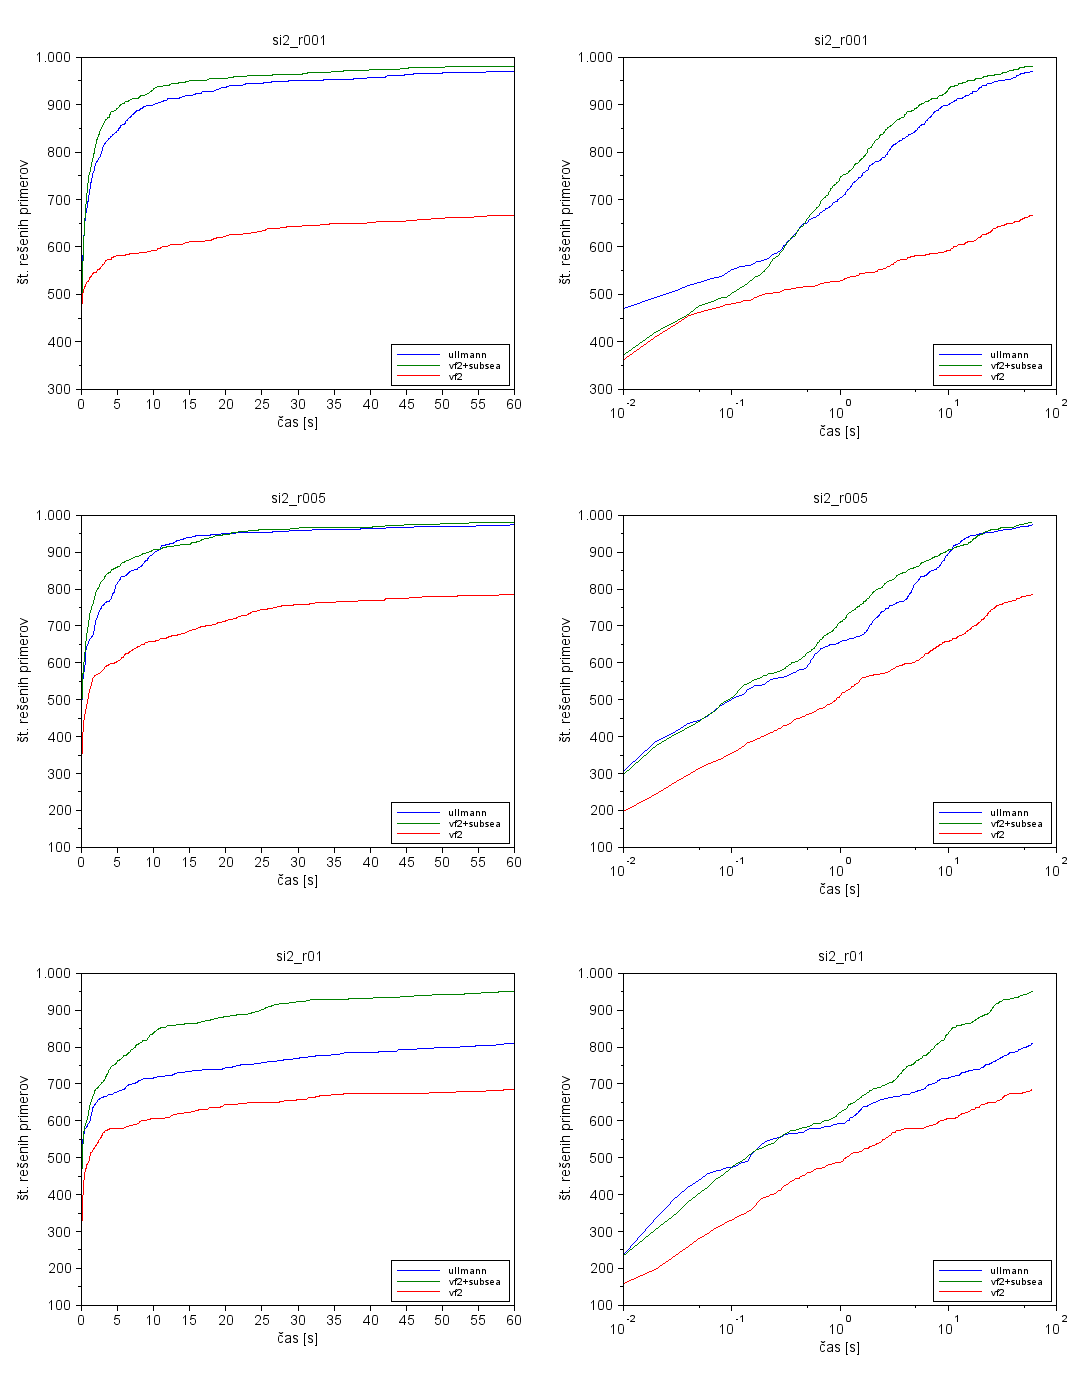
\includegraphics[width=15cm]{img/results_si2.png}
\end{center}
\caption{Število rešenih primerov za grafe tipov  si2\_r001, si2\_r005 in si2\_r01.}
\label{pic_res_si2}
\end{figure}

\begin{figure}
\begin{center}
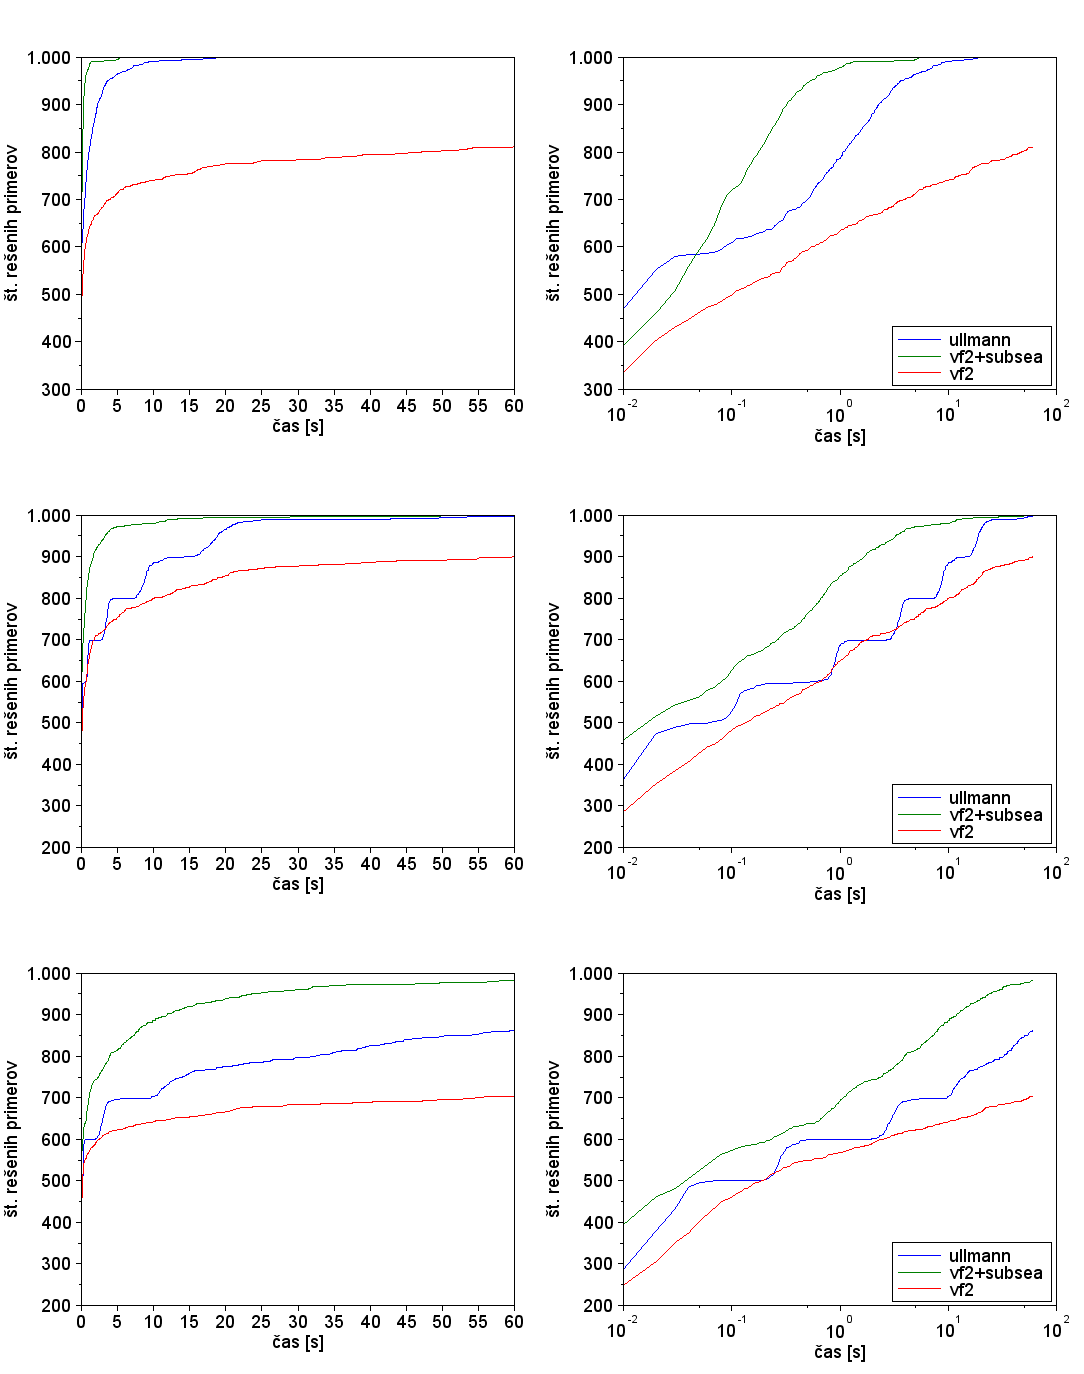
\includegraphics[width=15cm]{img/results_si4.png}
\end{center}
\caption{Število rešenih primerov za grafe tipov si4\_r001, si4\_r005, si4\_r01.}
\label{pic_res_si4}
\end{figure}

\begin{figure}
\begin{center}
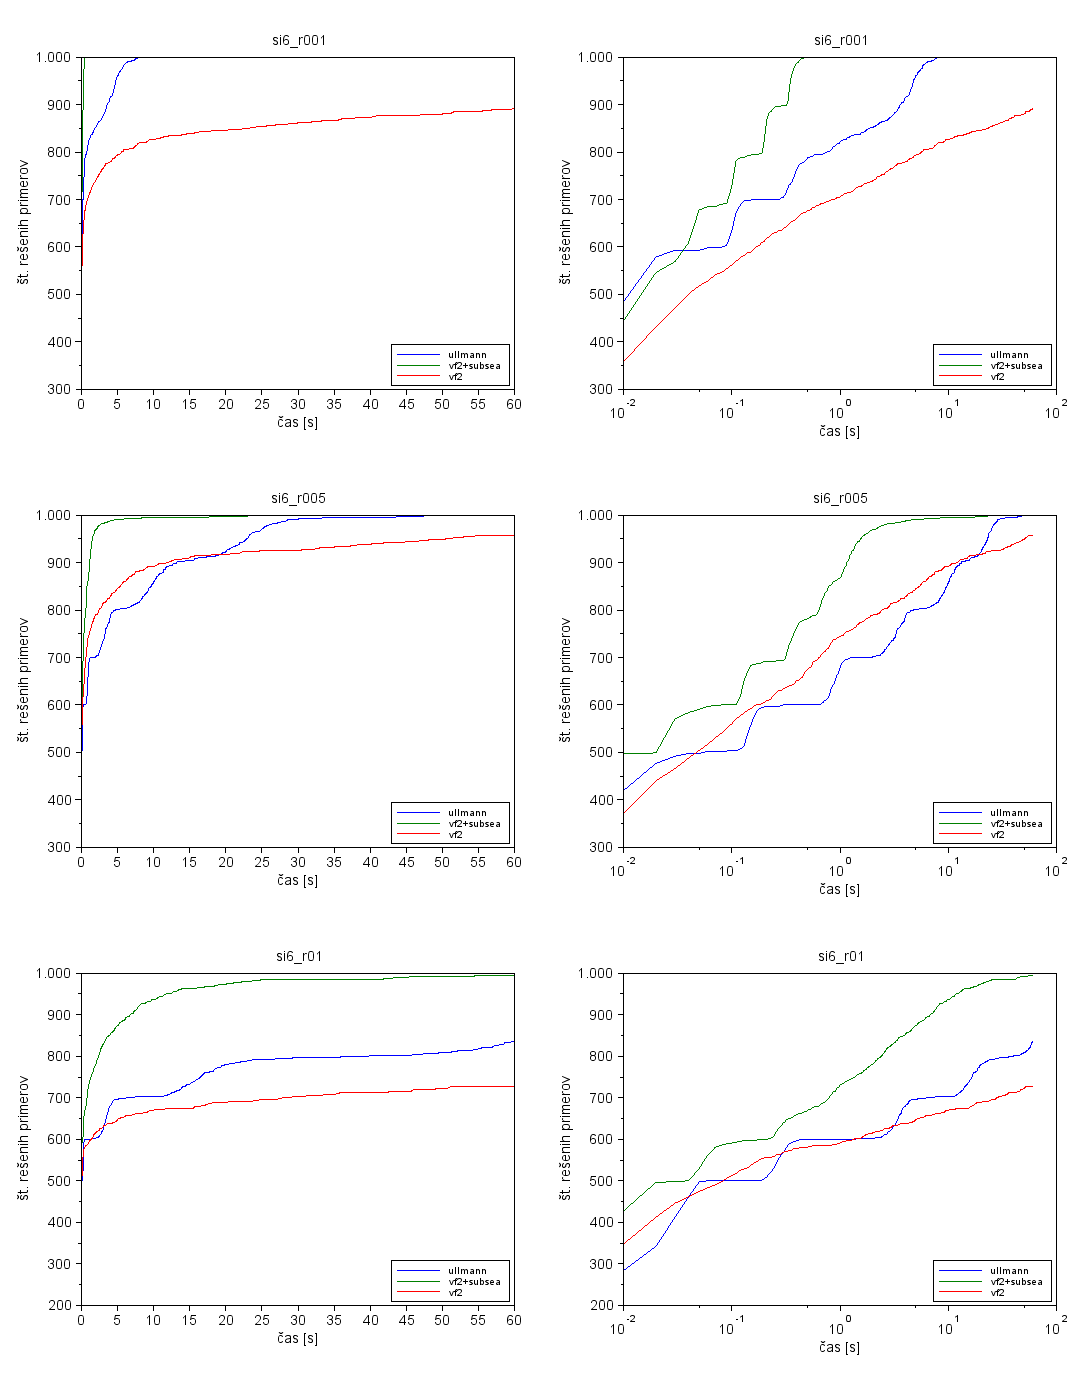
\includegraphics[width=15cm]{img/results_si6.png}
\end{center}
\caption{Število rešenih primerov za grafe tipov si6\_r001, si6\_r005 in si6\_r01.}
\label{pic_res_si6}
\end{figure}


\begin{figure}
\begin{center}
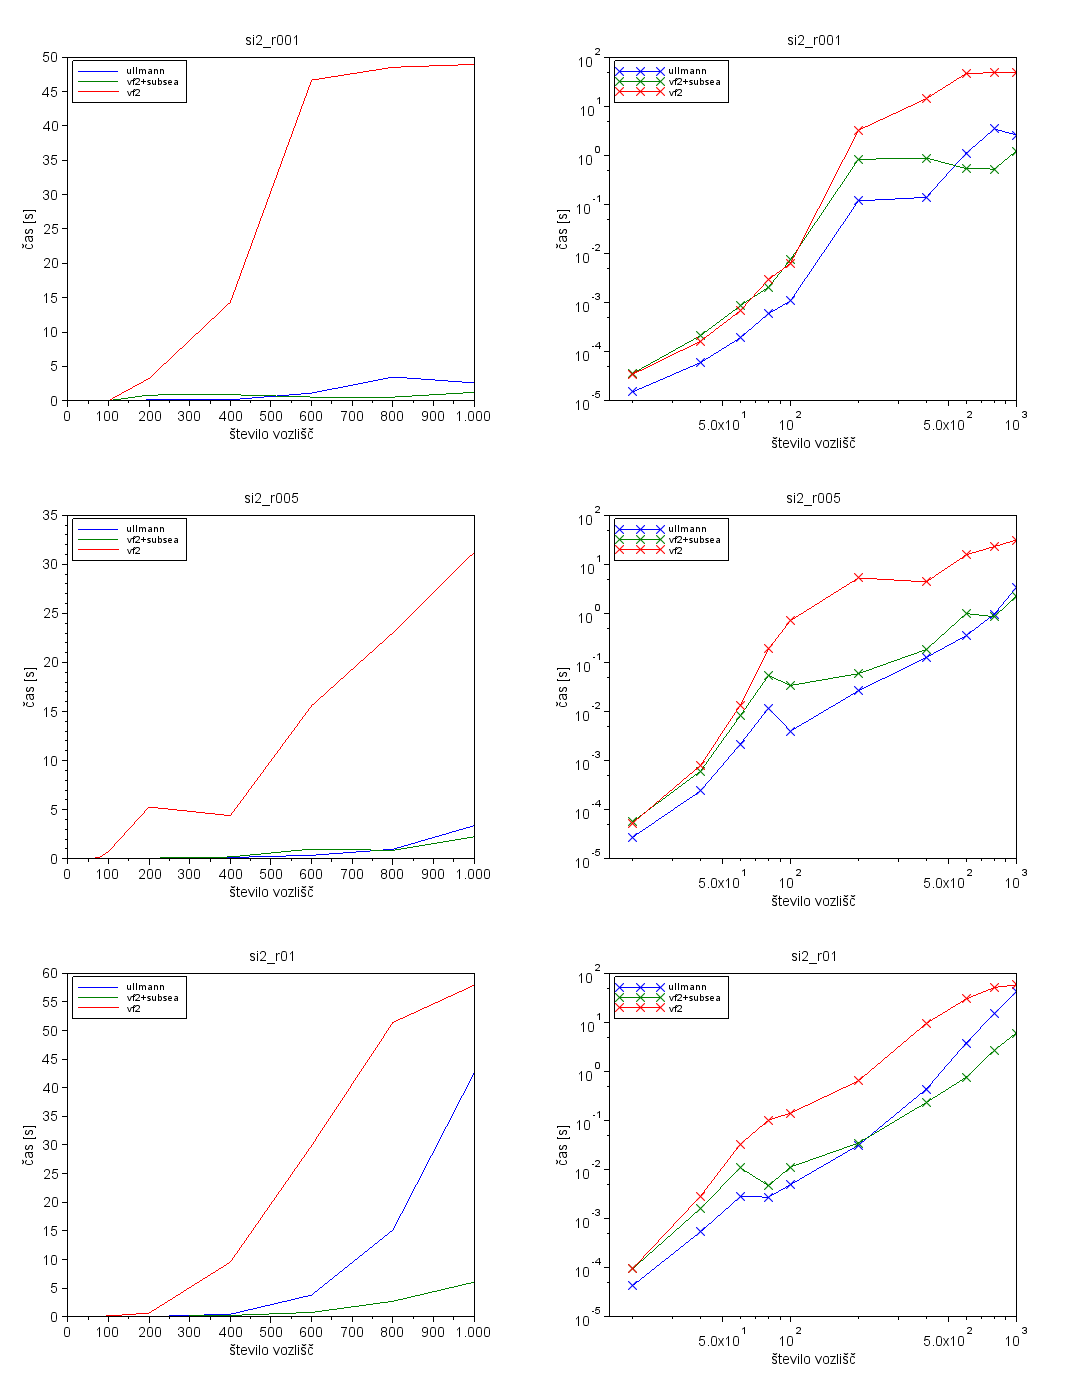
\includegraphics[width=15cm]{img/results2_si2.png}
\end{center}
\caption{Povprečen čas reševanja za grafe tipov si2\_r001, si2\_r005 in si2\_r01.}
\label{pic_res2_si2}
\end{figure}

\begin{figure}
\begin{center}
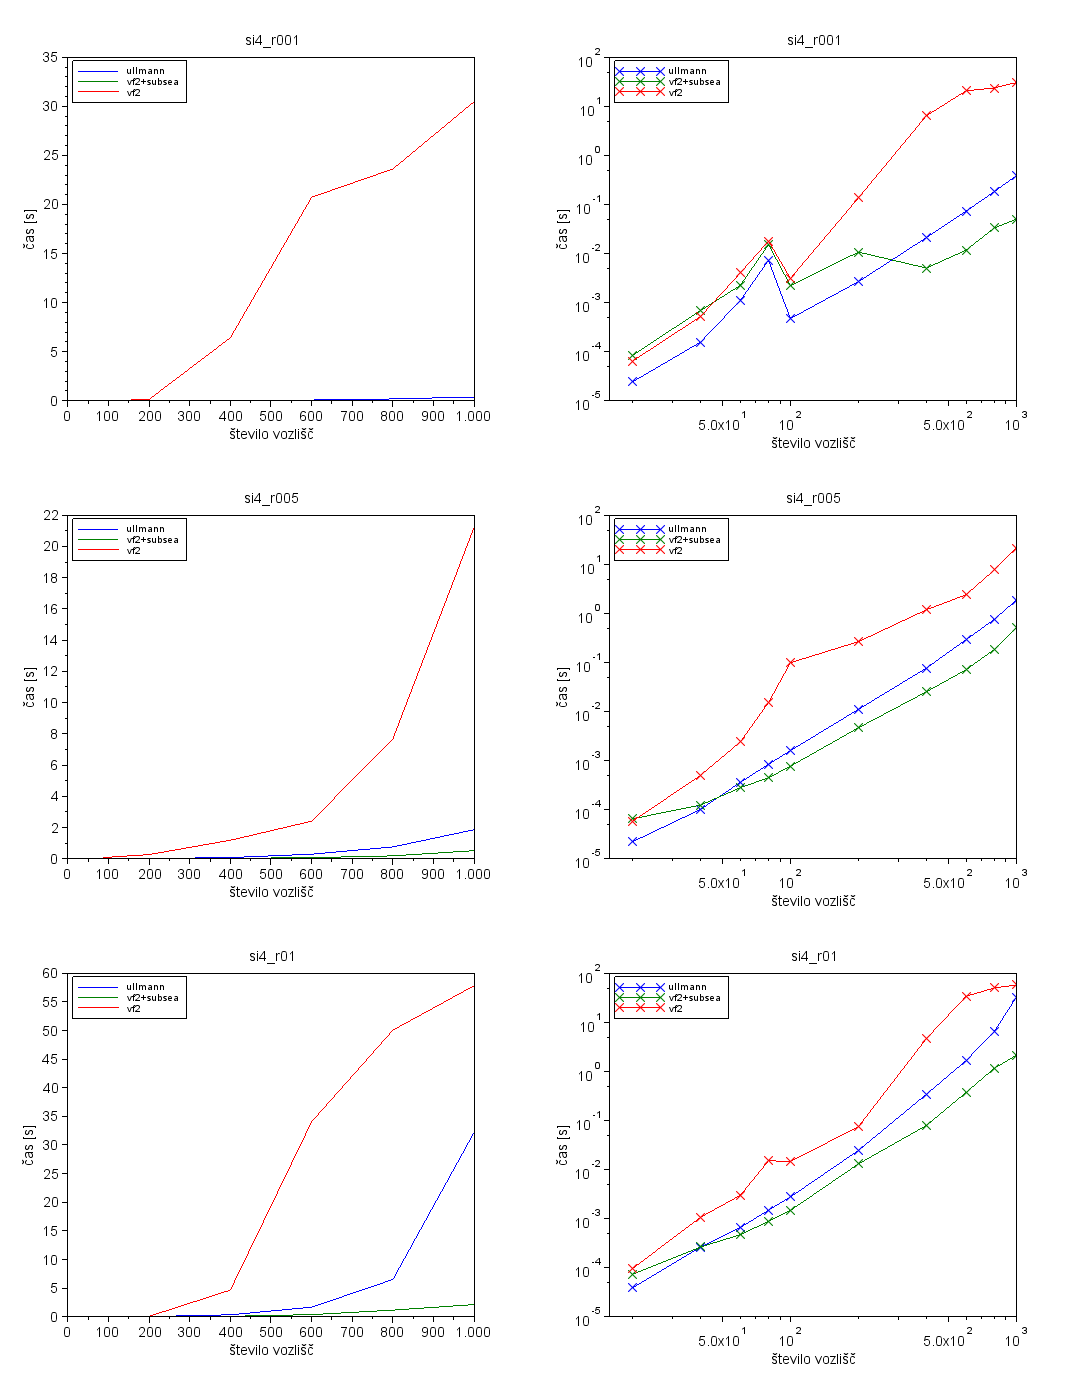
\includegraphics[width=15cm]{img/results2_si4.png}
\end{center}
\caption{Povprečen čas reševanja za grafe tipov si4\_r001, si4\_r005, si4\_r01.}
\label{pic_res2_si4}
\end{figure}

\begin{figure}
\begin{center}
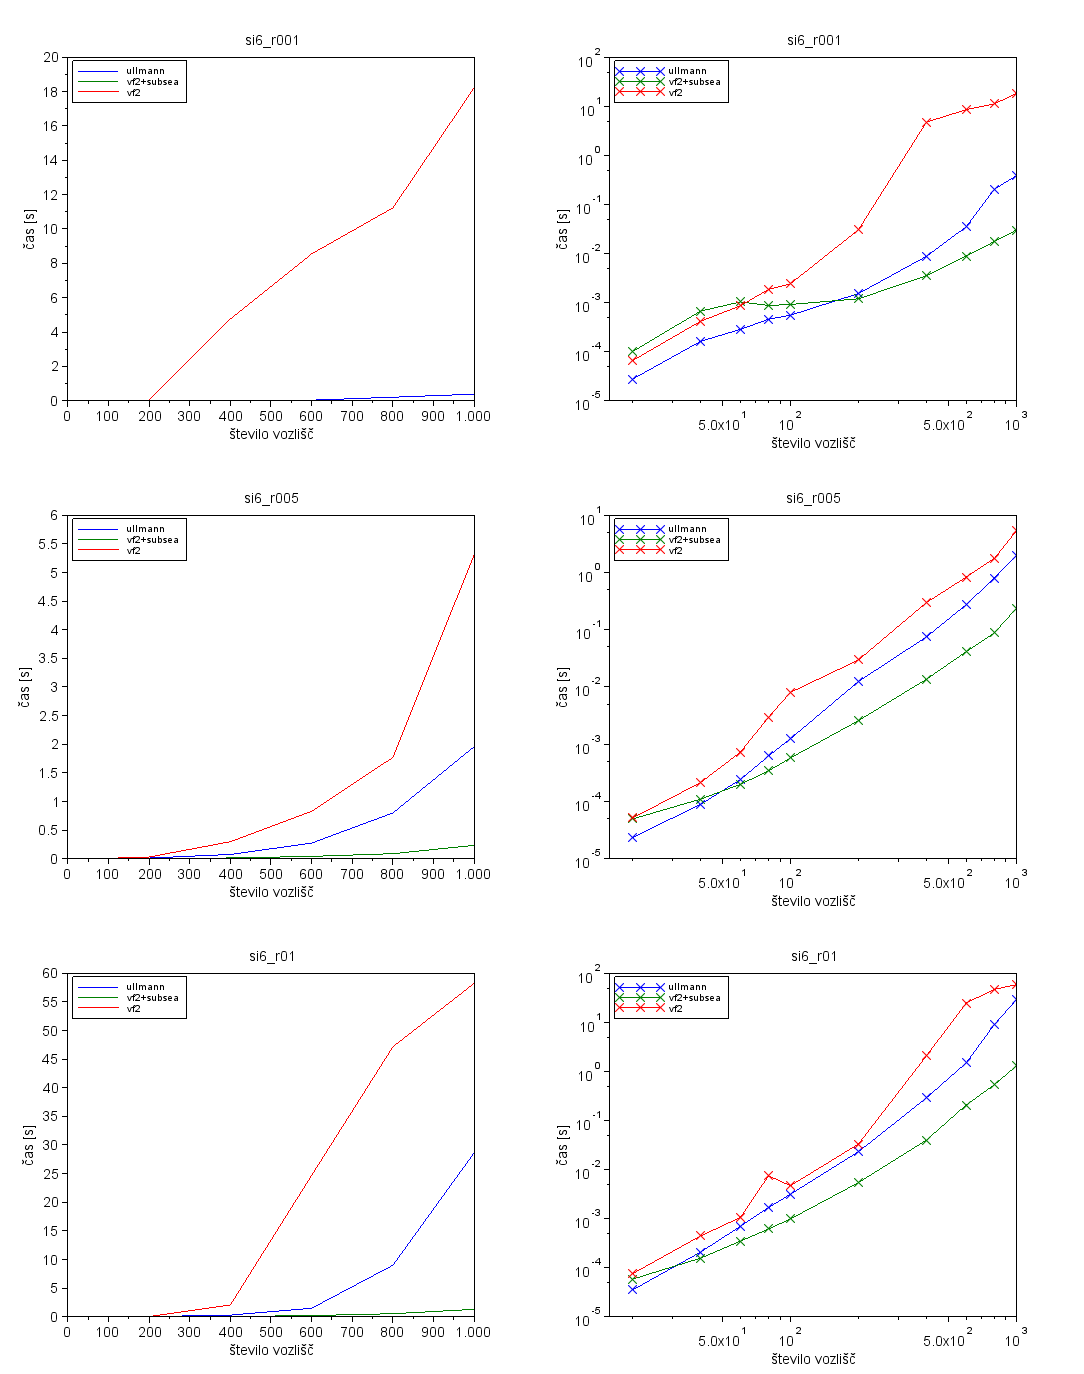
\includegraphics[width=15cm]{img/results2_si6.png}
\end{center}
\caption{Povprečen čas reševanja za grafe tipov si6\_r001, si6\_r005 in si6\_r01.}
\label{pic_res2_si6}
\end{figure}




\chapter{Sklepne ugotovitve}

	V delu smo primerjali tri algoritme za iskanje izomorfnih podgrafov in jih preizkusili na bazi 9000 parov grafov. Na manjših testnih primerih je najhitrejši
	izboljšani Ullmannov algoritem, kar ima praktično vrednost npr. pri iskanju na kemijskih grafih -- ti so običajno majhni, iskati pa je potrebno v velikih
	bazah grafov~\cite{chem}. Na večjih grafih in na grafih z več povezavami je boljši algoritem, ki smo ga ustvarili sami kot kombinacijo algoritma VF2
	in algoritma Subsea. Oba izboljšana algoritma sta vsaj za velikostni red hitrejša od obstoječega VF2, ki je trenutno najbolj uporabljan algoritem v praksi.
	
	Naslednji korak bi bila implementacija celotnega algoritma Subsea. Preveriti je potrebno, če se tudi celoten algoritem obnaša podobno kot hibrid med
	VF2 in Subsea. Lahko bi poskusili tudi obratno od naše izboljšave, torej da bi v algoritmu Subsea uporabili dele algoritma VF2. Konkretno bi lahko v
	fazi iskanja uporabili preverjanje kandidatov iz VF2 (opisano v razdelku~\ref{vf2:feasible}). Subsea namreč preverja samo kandidatove že preiskane
	sosede, VF2 pa z relativno majhnim vplivom na čas računanja preveri tudi neobiskane sosede. Preverili bi lahko tudi možnost vzporednega računanja
	opisanih algoritmov.

	Algoritme bi morali preizkusiti tudi na več testnih primerih. Najprej na preostalih grafih iz uporabljene baze grafov, potem pa še na realnih grafih iz
	prakse kot so npr. proteinih in socialna omrežja.
% praktični potencial


	
\clearemptydoublepage
\renewcommand{\baselinestretch}{1.0} % ustrezen razmik med vrsticami
\appendix
	\chapter {Implementacija izboljšave algoritma VF2}
	\label{appendix1}
		\begin{lstlisting}[frame=tb, caption={Zgodovina pregleda grafa za algoritem VF2 (vflib)}, label={app_vf2+sub}]	
#include <algorithm>
#include <vector>
#include <cstdio>
#include <climits>
#include <cstring>
#include <iostream>
#include "argraph.h"

// This class calculates order as described in Subsea algorithm - 
// depth first search and choose best with breadth first search
class SearchTraverse {
private:
	int n;
	node_id* order;
	bool *processed;
	bool *estimateProcessed;
	int index;
	Graph *g;

	struct NodeEstimate {
		node_id id;
		int steps;
		int size;
	};

	// a < b
	bool nodeEstimateCompare(NodeEstimate a, NodeEstimate b) {
		if (a.steps == b.steps) {
			return a.size < b.size;
		} else {
			return a.steps < b.steps;
		}
	}

	// Breadth first search
	NodeEstimate getNodeEstimate(node_id start, node_id from) {
		memset(estimateProcessed, 0, sizeof(bool) * n);
		NodeEstimate e;
		e.id = start;
		e.steps = 1;
		e.size = 0;
		int total = 0;
		std::vector<node_id> s;
		std::vector<node_id> n;
		s.push_back(start);
		do {
			int p = 0;
			bool skippedEdge = false;
			// Loop visited nodes
			for (unsigned int idx = 0; idx < s.size(); idx++) {
				// Loop node neighbors
				for (int i = 0; i < g->InEdgeCount(s.at(idx)); i++) {
					node_id n1 = g->GetInEdge(s.at(idx), i);
					if (s.at(idx) == start && n1 == from && skippedEdge == false) {	// Do not use edge start->from
						skippedEdge = true; // Only skip one edge
						continue;
					}
					if (!estimateProcessed[n1]) { // Add to visited
						n.push_back(n1);
						estimateProcessed[n1] = true;
						if (processed[n1])
							p++;	// Count, if node is in goal
					}
				}
				for (int i = 0; i < g->OutEdgeCount(s.at(idx)); i++) {
					node_id n1 = g->GetOutEdge(s.at(idx), i);
					if (s.at(idx) == start && n1 == from && skippedEdge == false) {
						skippedEdge = true;
						continue;
					}
					if (!estimateProcessed[n1]) {
						n.push_back(n1);
						estimateProcessed[n1] = true;
						if (processed[n1])
							p++;
					}
				}
			}
			if (p > 0) {
				e.size = -p;
				return e;
			} else {
				e.steps++;
				total += n.size();
				s.clear();
				s.swap(n);
			}
		} while (s.size() > 0);
		e.steps = 99999999;
		e.size = total;
		return e;
	}

	// Depth first visit, in best-first order
	void Visit(node_id node) {
		order[index++] = node;
		processed[node] = true;
		
		// Find all non-processed neighbors of added node
		std::vector<node_id> neighbors;
		for (int i = 0; i < g->InEdgeCount(node); i++) {
			node_id n1 = g->GetInEdge(node, i);
			if (!processed[n1]) {
				neighbors.push_back(n1);
			}
		}
		for (int i = 0; i < g->OutEdgeCount(node); i++) {
			node_id n1 = g->GetOutEdge(node, i);
			if (!processed[n1]) {
				neighbors.push_back(n1);
			}
		}

		// Visit all neighbors in best-first order
		while (neighbors.size() > 0) {
			int bestNodeIdx = -1;
			node_id bestNode = NULL_NODE;
			NodeEstimate bestEstimate;

			// Find best neighbor
			for (unsigned int i = 0; i < neighbors.size(); i++) {
				node_id n1 = neighbors.at(i);
				if (!processed[n1]) {
					NodeEstimate nEstiname = getNodeEstimate(n1, node);
					if (bestNode == NULL_NODE || nodeEstimateCompare(nEstiname, bestEstimate)) {
						bestNodeIdx = i;
						bestNode = n1;
						bestEstimate = nEstiname;
					}
				}
			}
			if (bestNode != NULL_NODE) {
				Visit(bestNode);
				// Remove visited neighbor
				neighbors[bestNodeIdx] = neighbors[neighbors.size()-1];
				neighbors.pop_back();
			} else {
				break;	// No more unvisited neighbors
			}
		}
	}

public:
	node_id * SortNodesBySearchTraverse(Graph *g) {
		n = g->NodeCount();
		order = new node_id[n];
		processed = new bool[n];
		estimateProcessed = new bool[n];
		index = 0;
		this->g = g;
		for (int i = 0; i < n; i++) {
			order[i] = NULL_NODE;
			processed[i] = false;
		}
		// Start with highest degree node (not part of Subsea)
		while (index < n) {
			int first = -1;
			int firstEdgeCnt = -1;
			for (int i = 0; i < n; i++) {
				if (!processed[i] && g->EdgeCount(i) > firstEdgeCnt) {
					first = i;
					firstEdgeCnt = g->EdgeCount(i);
				}
			}
			Visit(first);
		}
		delete[] processed;
		delete[] estimateProcessed;
		return order;
	}
};
	\end{lstlisting}
	
\clearpage
	\begin{lstlisting}[frame=tb, caption={Sprememba kode v knjižnici vflib za vključitev izboljšave algoritma VF2; \texttt{heuristicOrder} je vrnjena tabela iz	
	algoritma~\ref{app_vf2+sub}}, label={app_vf2+sub1}]
	bool VF2SubState::NextPair(node_id *pn1, node_id *pn2, node_id prev_n1, node_id prev_n2) {
	prev_n1 = heuristicOrder[core_len];
	if (prev_n2 == NULL_NODE)
		prev_n2 = 0;
	else
		prev_n2++;

	if (out_1[prev_n1] != 0 && in_1[prev_n1] != 0) {
		while (prev_n2 < n2 && (core_2[prev_n2] != NULL_NODE || out_2[prev_n2] == 0 || in_2[prev_n2] == 0)) {
			prev_n2++;
		}
	} else if (out_1[prev_n1] != 0) {
		while (prev_n2 < n2 && (core_2[prev_n2] != NULL_NODE || out_2[prev_n2] == 0)) {
			prev_n2++;
		}
	} else if (in_1[prev_n1] != 0) {
		while (prev_n2 < n2 && (core_2[prev_n2] != NULL_NODE || in_2[prev_n2] == 0)) {
			prev_n2++;
		}
	} else {
		while (prev_n2 < n2 && core_2[prev_n2] != NULL_NODE) {
			prev_n2++;
		}
	}

	if (prev_n1 < n1 && prev_n2 < n2) {
		*pn1 = prev_n1;
		*pn2 = prev_n2;
		return true;
	}

	return false;
}
	\end{lstlisting}


\begin{thebibliography}{99}

	%@article{LipetsVG09,
	%  title = {Subsea: an efficient heuristic algorithm for subgraph isomorphism},
	%  author = {Vladimir Lipets and Natalia Vanetik and Ehud Gudes},
	%  year = {2009},
	%  doi = {http://dx.doi.org/10.1007/s10618-009-0132-7},
	%  researchr = {http://researchr.org/publication/LipetsVG09},
	%  cites = {0},
	%  citedby = {0},
	%  journal = {Data Min. Knowl. Discov.},
	%  volume = {19}, %številka?
	%  number = {3}, % zvezek?
	%  pages = {320-350},
	%}

%@article{doi:10.1142/S0218001404003228,
%author = {CONTE, D. and FOGGIA, P. and SANSONE, C. and VENTO, M.},
%title = {THIRTY YEARS OF GRAPH MATCHING IN PATTERN RECOGNITION},
%journal = {International Journal of Pattern Recognition and Artificial Intelligence},
%volume = {18},
%number = {03},
%pages = {265-298},
%year = {2004},
%doi = {10.1142/S0218001404003228},

	\bibitem{thirtyyears} D.~Conte, P.~Foggia, C.~Sansone, M.~Vento, ``Thirty Years Of Graph Matching In Pattern Recognition",
		\textit{International Journal of Pattern Recognition and Artificial Intelligence}, št.~18, zv.~3, 2004, str.~265--298

	\bibitem{vf2} L.~Cordella, P.~Foggia, C.~Sansone, M.~Vento, ``A (Sub)Graph Isomorphism Algorithm for Matching Large Graphs",
		\textit {IEEE Trans. Pattern Analysis and Machine Intelligence}, št.~26, zv.~10, 2004, str.~1367--1372.
		
	\bibitem{vf2_3} L.~Cordella, P.~Foggia, C.~Sansone, M.~Vento, ``An improved algorithm for matching large graphs",
		\textit {3rd IAPR-TC15 Workshop on Graph-based Representations in Pattern Recognition, Cuen}, 2001, str.~149--159.
		
	\bibitem{vf2_2} L.~Cordella, P.~Foggia, C.~Sansone, M.~Vento, ``Performance evaluation of the VF graph matching algorithm",
		%\textit {Proc. Int. Conf Image Analysis and Processing}, 1999, str.~1372--1177.
		\textit {Proceedings of the 10th International Conference on Image Analysis and Processing}, 1999, str.~1372--1177.

	\bibitem{chem} H.~C.~Ehrlich, M.~Rarey, ``Systematic benchmark of substructure search in molecular graphs - From Ullmann to VF2",
		\textit{Journal of Cheminformatics}, št.~4, zv.~1, 2012

	\bibitem{database} P.~Foggia, C.~Sansone, M.~Vento, ``A Database of Graphs for Isomorphism and Sub-Graph Isomorphism Benchmarking",
		\textit{CoRR}, 2001, str.~176--187
		
	\bibitem{npcomplete} M.~R.~Garey, D.~S.~Johnson, ``Computers and Intractability: A Guide to the Theory of NP-Completeness",
		Freeman and Company, 1979.
	
	\bibitem{indepth}J.~Lee, W.~Han, R.~Kasperovics, J.~Lee, ``An In-depth Comparison of Subgraph Isomorphism Algorithms in Graph Databases"
		\textit{Proceedings of the VLDB Endowment (PVLDB)}, št.~6, zv.2, 2012, str. 133--144
	
	\bibitem{subsea} V.~Lipets, N.~Vanetik, E.~Gudes, ``Subsea: an efficient heuristic aglorithm for subgraph isomorphism",
		\textit{Data Mining and Knowledge Discovery}, št.~19, zv.~3, 2009, str.~320--350.

	\bibitem{poly} B.~T.~Messmer, H.~Bunke, ``Subgraph isomorphism detection in polynomial time on preprocessed model graphs",
		\textit{Recent Developments in Computer Vision}, 1996, str.~373--382

	\bibitem{ull+} J. Mihelič, U. Čibej, ``Izboljšave Ullmannovega algoritma za problem iskanja podgrafnih izomorfizmov",
		\textit{Zbornik enaindvajsete mednarodne Elektrotehniške in računalniške konference ERK}, 2012

	\bibitem{alldiff} C.~Solnon, ``AllDifferent-based filtering for subgraph isomorphism",
		\textit{Artificial Intelligence}, št.~174, zv.~12--13, 2010, str.~850--864

	% Journal of the ACM, Vol. 23, No. 1. (January 1976), pp. 31-42
	\bibitem{ullmann} J.~R.~Ullmann, ``An Algorithm for Subgraph Isomorphism",
		\textit{Journal of the ACM}, št.~23, zv.~1, 1976, str.~31--42.

	\bibitem{zampelli-th} S.~Zamplelli, ``A constraint programming approcah to subgraph isomorphism", Doktorska disertacija, 
	Universit\'{e} catholique de Louvain, D\'{e}partement d’Ing\'{e}nierie Informatique, Belgija, 2008.
	

\end{thebibliography}


\end{document}

